% main.tex — Artisync: Plataforma web de intermediación entre creadores de
% contenido digital y clientes con estrategia híbrida de acceso a datos,
% verificación asistida por IA y evaluación empírica multidimensional
%
% Proyecto de Fin de Curso (PFC) — UTEQ, Facultad de Ciencias de la
% Computación y Diseño Digital, Ingeniería de Software.
%
% Compilación (ver README.md de esta carpeta para el detalle):
%   latexmk -pdf -bibtex main.tex
% o manualmente:
%   pdflatex main.tex && bibtex main && pdflatex main.tex && pdflatex main.tex
%
% Estilo de citas: IEEE numérico (\bibliographystyle{ieeetr}), referencias
% en referencias.bib. No requiere la clase IEEEtran (se decidió reporte
% académico de una columna, ver README.md, "¿Por qué no IEEEtran?").

\documentclass[12pt,a4paper,oneside]{report}

% ---------- Idioma y codificación ----------
\usepackage[utf8]{inputenc}
\usepackage[T1]{fontenc}
\usepackage[spanish,es-noindentfirst]{babel}
\usepackage{lmodern}

% ---------- Página y espaciado ----------
\usepackage[margin=2.5cm]{geometry}
\usepackage{setspace}
\onehalfspacing

% ---------- Justificación: evita que rutas de archivo largas en \texttt{}
% (sin puntos de guion natural) se salgan del margen derecho ----------
\usepackage{microtype}
\sloppy
\emergencystretch=3em
\tolerance=2000
\usepackage[htt]{hyphenat}

% ---------- Tablas, figuras, código ----------
\usepackage{graphicx}
\usepackage{tikz}
\usetikzlibrary{babel}
\usepackage{booktabs}
\usepackage{longtable}
\usepackage{array}
\usepackage{caption}
\usepackage{subcaption}
\usepackage{listings}
\usepackage{xcolor}
\usepackage{float}

% ---------- Matemáticas y símbolos ----------
\usepackage{amsmath}
\usepackage{amssymb}

% ---------- Citas IEEE + hipervínculos ----------
\usepackage{cite}
\usepackage[hidelinks,breaklinks]{hyperref}
\usepackage{url}
\Urlmuskip=0mu plus 1mu

% ---------- Encabezados ----------
\usepackage{fancyhdr}
\pagestyle{fancy}
\fancyhf{}
\fancyhead[LE,RO]{\thepage}
\fancyhead[RE]{\nouppercase{\leftmark}}
\fancyhead[LO]{\nouppercase{\rightmark}}
\renewcommand{\headrulewidth}{0.4pt}
\setlength{\headheight}{14.5pt}

% ---------- Títulos de capítulo ----------
\usepackage{titlesec}
\titleformat{\chapter}[hang]{\normalfont\huge\bfseries}{\thechapter.}{20pt}{\Huge}
\titlespacing*{\chapter}{0pt}{0pt}{30pt}

% ---------- Acrónimos ----------
\usepackage[acronym,nomain]{glossaries}
\makeglossaries

\newacronym{adr}{ADR}{Architecture Decision Record}
\newacronym{api}{API}{Application Programming Interface}
\newacronym{ci}{CI}{Continuous Integration}
\newacronym{crud}{CRUD}{Create, Read, Update, Delete}
\newacronym{dsr}{DSR}{Design Science Research}
\newacronym{gqm}{GQM}{Goal-Question-Metric}
\newacronym{ic}{IC}{Intervalo de Confianza}
\newacronym{imrad}{IMRaD}{Introduction, Methods, Results and Discussion}
\newacronym{jpa}{JPA}{Jakarta Persistence API}
\newacronym{jwt}{JWT}{JSON Web Token}
\newacronym{moscow}{MoSCoW}{Must, Should, Could, Won't}
\newacronym{orm}{ORM}{Object-Relational Mapping}
\newacronym{owasp}{OWASP}{Open Web Application Security Project}
\newacronym{pfc}{PFC}{Proyecto de Fin de Curso}
\newacronym{pitr}{PITR}{Point-In-Time Recovery}
\newacronym{rbac}{RBAC}{Role-Based Access Control}
\newacronym{rpo}{RPO}{Recovery Point Objective}
\newacronym{rto}{RTO}{Recovery Time Objective}
\newacronym{srs}{SRS}{Software Requirements Specification}
\newacronym{sp}{SP}{Stored Procedure (Procedimiento Almacenado)}
\newacronym{sus}{SUS}{System Usability Scale}
\newacronym{totp}{TOTP}{Time-based One-Time Password}
\newacronym{wal}{WAL}{Write-Ahead Log}

% ---------- Macro de honestidad: marca visualmente los puntos que el
% equipo todavía debe resolver, en vez de ocultarlos o inventarlos ----------
\newcommand{\pendiente}[1]{%
  \textbf{\textcolor{purple}{[PENDIENTE ---~#1]}}%
}

% ---------- Entorno para bloques de listados con numeración propia ----------
\lstdefinestyle{codebase}{
  basicstyle=\ttfamily\footnotesize,
  breaklines=true,
  columns=fullflexible,
  frame=single,
  numbers=left,
  numberstyle=\tiny,
  keywordstyle=\color{blue!60!black}\bfseries,
  commentstyle=\color{gray},
  stringstyle=\color{orange!70!black},
  showstringspaces=false,
  tabsize=2
}
\lstset{style=codebase}

\graphicspath{{../diagramas/}{../mediciones/}{../mediciones/sus/}}

\title{Artisync: Plataforma web de intermediación entre creadores de
contenido digital y clientes con estrategia híbrida de acceso a datos,
verificación asistida por IA y evaluación empírica multidimensional}
\author{Bone Arroyo, Niurca Scarleth \and Carvajal Loor, Johan Stalin \and
Figueroa Morales, Bryan Javier \and Rios Cuyabazo, Jhon Kevin}
\date{17 de agosto de 2026}

\begin{document}

\pagenumbering{roman}
% 00-portada-resumen.tex — Portada, resúmenes ES/EN, metadatos de la entrega.
% Fuente: docs/informe-final (borrador previo), verificado contra
% CONTRIBUTORS.md, README.md, CITATION.cff y docs/observaciones/.

\begin{titlepage}
\centering

\textsc{\Large Universidad Técnica Estatal de Quevedo}\\[0.3cm]
\textsc{\large Facultad de Ciencias de la Computación y Diseño Digital}\\
\textsc{\large Carrera de Ingeniería de Software}\\[1.5cm]

\rule{\linewidth}{0.5mm}\\[0.4cm]
{\LARGE \bfseries ARTISYNC: Plataforma web de intermediación entre
creadores de contenido digital y clientes con estrategia híbrida de acceso
a datos, verificación asistida por IA y evaluación empírica
multidimensional}\\[0.4cm]
\rule{\linewidth}{0.5mm}\\[1cm]

{\large \gls{pfc} --- Aplicaciones Web, Quinto Nivel}\\
{\large Período Académico Presencial 2026-2027}\\[1.5cm]

\begin{minipage}{0.9\textwidth}
\centering
\begin{tabular}{@{}ll@{}}
\toprule
\textbf{Integrante} & \textbf{ORCID} \\
\midrule
Bone Arroyo, Niurca Scarleth & \url{https://orcid.org/0009-0002-2219-2800} \\
Carvajal Loor, Johan Stalin & \url{https://orcid.org/0009-0008-9229-382X} \\
Figueroa Morales, Bryan Javier & \url{https://orcid.org/0009-0009-6357-4996} \\
Rios Cuyabazo, Jhon Kevin & \url{https://orcid.org/0009-0003-7446-9450} \\
\bottomrule
\end{tabular}
\end{minipage}\\[1cm]

\textbf{Docente-director:} Dr. Gleiston Cicerón Guerrero Ulloa, Ph.D.\\
\texttt{gguerrero@uteq.edu.ec}\\[1cm]

\begin{minipage}{0.85\textwidth}
\centering
\textbf{Fecha de cierre:} 11 de septiembre de 2026 (semana 19)\\
\textbf{Etiqueta del artefacto:} \texttt{v1.0.0}\\
\textbf{DOI del software (Zenodo):} \texttt{10.5281/zenodo.21978572}
(archivo de \texttt{v1.0.0}; la versión anterior, \texttt{v0.9.0-rc},
quedó archivada aparte en \texttt{10.5281/zenodo.21730559})\\
\textbf{DOI del dataset de mediciones (Zenodo):}
\texttt{10.5281/zenodo.22236251} (depósito separado del software,
licencia CC~BY~4.0, conforme al Bloque D.3 de la guía)
\end{minipage}

\vfill
{\small Repositorio: \url{https://github.com/JohanCarvajal04/Proyecto-WEB-ARTISYNC}}
\end{titlepage}

\chapter*{Resumen}
\addcontentsline{toc}{chapter}{Resumen}

\textbf{Contexto y problema.} La economía creativa digital fragmenta la contratación, comunicación y pagos entre plataformas desconectadas, aumentando el riesgo de fraude. \textbf{Objetivo.} Diseñar, implementar y evaluar Artisync, plataforma construida sobre Spring Boot y Angular que integra el ciclo completo de intermediación con pagos \emph{escrow}, usando una estrategia híbrida de acceso a datos (\gls{orm} y PL/pgSQL) y verificación por IA. \textbf{Métodos.} Se aplicó la metodología \gls{dsr} de Peffers~\cite{PEFFERS2007}, ingeniería de requisitos ISO/IEC/IEEE~29148:2018~\cite{ISO29148}, y evaluación empírica de rendimiento (k6), seguridad (controles OWASP Top 10 y análisis dinámico con ZAP), usabilidad (\gls{sus}, $N=16$)~\cite{BROOKE1996,BANGOR2009}, cobertura (JaCoCo) y calidad web (Lighthouse), sobre un entorno reproducible con Docker Compose, con comparaciones de rendimiento validadas mediante pruebas inferenciales no paramétricas y tamaño de efecto ordinal. \textbf{Resultados principales.} Artisync logró p95 de 50.17~ms bajo carga, 0\,\% de errores HTTP, cobertura JaCoCo de 82.93\,\% líneas y 71.50\,\% ramas ---las tres capas sobre el umbral de 70\,\%---, Lighthouse Performance 100/100 (desktop) y 80 (mobile), y 0 hallazgos altos en ZAP. La usabilidad, en cambio, alcanzó un \gls{sus} de 61.25/100, sin superar el umbral de aceptabilidad (68). Se implementaron 26 procedimientos almacenados sin SQL dinámico, y los 37 requisitos declarados conservan trazabilidad automática hacia código y pruebas, validada en \gls{ci}. \textbf{Conclusiones.} Artisync demuestra la viabilidad de la estrategia híbrida y de la validación asistida por IA en 17 semanas, con evidencia reproducible; la usabilidad es la única dimensión que no alcanza su umbral y concentra el trabajo futuro.

\textbf{Palabras clave:} ingeniería de requisitos; procedimientos
almacenados; verificación de identidad; arquitectura de microservicios;
usabilidad de software; seguridad web

\chapter*{Abstract}
\addcontentsline{toc}{chapter}{Abstract}

\textbf{Context and problem.} The digital creative economy fragments contracting, communication, and payments across disconnected platforms, increasing fraud risks. \textbf{Objective.} To design, implement, and evaluate Artisync, a platform built on Spring Boot and Angular integrating the intermediation cycle with escrow payments, a hybrid data-access strategy (ORM and PL/pgSQL), and AI-assisted verification. \textbf{Methods.} Peffers' \gls{dsr} methodology~\cite{PEFFERS2007} was applied, alongside ISO/IEC/IEEE~29148:2018 requirements engineering~\cite{ISO29148}, and empirical evaluations of performance (k6), security (OWASP Top 10 controls and dynamic scanning with ZAP), usability (\gls{sus}, $N=16$)~\cite{BROOKE1996,BANGOR2009}, code coverage (JaCoCo), and web quality (Lighthouse), on an environment reproducible with Docker Compose, with performance comparisons validated through non-parametric inferential tests and ordinal effect sizes. \textbf{Main results.} Artisync achieved a p95 of 50.17~ms under load, 0\% HTTP errors, JaCoCo coverage of 82.93\% lines and 71.50\% branches ---all three layers above the 70\% threshold---, Lighthouse Performance 100/100 (desktop) and 80 (mobile), and 0 high security findings in ZAP. Usability, by contrast, reached a \gls{sus} of 61.25/100, failing to pass the acceptability threshold (68). 26 stored procedures free of dynamic SQL were implemented, and the 37 declared requirements maintain automated traceability to code and tests, validated in \gls{ci}. \textbf{Conclusions.} Artisync proves the viability of hybrid data access and AI-assisted validation in a 17-week timeframe, with reproducible evidence; usability is the only dimension falling short of its threshold and concentrates the future work.

\textbf{Keywords:} requirements engineering; stored procedures; identity
verification; microservices architecture; software usability; web
security


\newpage
\tableofcontents
\newpage
\listoffigures
\newpage
\listoftables
\newpage
\lstlistoflistings
\newpage
\printglossary[type=\acronymtype,title={Lista de siglas y acrónimos}]

\newpage
\pagenumbering{arabic}

% 01-introduccion.tex — Fuente: docs/informe-final/01-introduccion.md (borrador)

\chapter{Introducción}
\label{cap:introduccion}

\section{Contexto y motivación}

La economía creativa digital ---el conjunto de actividades económicas en
las que músicos, ilustradores, diseñadores y desarrolladores monetizan
directamente su trabajo a través de internet--- ha crecido de forma
sostenida como alternativa de ingreso para profesionales
independientes~\cite{PERES2024}. Sin embargo, la infraestructura que
sostiene esa economía sigue fragmentada: un creador independiente típico
coordina la comunicación con clientes por una red social o mensajería
instantánea, gestiona el cobro por una pasarela de pagos genérica sin
retención de garantía, y no cuenta con un mecanismo estandarizado de
contrato ni de verificación de identidad de ninguna de las dos partes.
Esta fragmentación introduce fricción operativa medible: la literatura
sobre freelancers de plataformas digitales reporta la gestión de múltiples
herramientas desconectadas y la ausencia de mecanismos de protección de
pago como fuentes recurrentes de conflicto y abandono de la
actividad~\cite{GUSSEK2023}. El patrón de pago en garantía (\emph{escrow})
---retener los fondos del cliente hasta la aprobación explícita del
entregable--- es la mitigación estándar de la industria para el riesgo de
incumplimiento en transacciones entre partes que no se conocen
previamente, formalizable incluso mediante protocolos de depósito dual
verificables~\cite{ASGAONKAR2019}, pero su implementación correcta exige
una arquitectura de datos con garantías transaccionales estrictas, que la
mayoría de las herramientas genéricas de mensajería y pago no ofrece de
forma nativa. 

Artisync responde a esa fragmentación con una plataforma que centraliza,
en un único sistema auditable, el ciclo completo de intermediación entre
\textbf{Creadores} de contenido digital y \textbf{Clientes}: perfil
verificado por un servicio de inteligencia artificial, catálogo dinámico
de servicios y productos, mensajería moderada que bloquea el intercambio
de datos de contacto externo (mitigación directa del riesgo de que las
partes se muevan fuera del sistema auditable), contrato con firma
electrónica generado desde plantilla, flujo de pedido por etapas con
trazabilidad completa, pago mediante PayPal Orders v2 con patrón
\emph{escrow}, y funciones sociales (seguidores, comentarios, sorteos)
para fomentar la retención de usuarios. El modelo de doble lado
(Creador/Cliente) de Artisync es, en esencia, una plataforma multilateral
en el sentido de Hagiu y Wright~\cite{HAGIU2015}, orquestando transacciones
entre dos grupos de usuarios que de otro modo dependerían de
intermediarios genéricos.

\section{Preguntas de investigación}

\textbf{RQ1.} ¿Cumple el sistema, con evidencia empírica reproducible, los
umbrales de rendimiento, seguridad, usabilidad, cobertura de código y
calidad web declarados como requisitos no funcionales de la especificación
(\texttt{docs/requisitos/SRS.md})?

\textbf{RQ2.} ¿Es la estrategia híbrida de acceso a datos (operaciones
CRUD elementales vía ORM, operaciones multi-tabla vía procedimientos
almacenados PL/pgSQL invocados exclusivamente mediante los mecanismos
formales de JPA~2.1) implementable y verificable end-to-end dentro de las
restricciones de tiempo y equipo de un proyecto académico de 17 semanas,
sin introducir vulnerabilidades de inyección SQL?

\textbf{RQ3.} ¿En qué medida el proceso de ingeniería de requisitos
aplicado (elicitación, negociación, documentación y validación según el
marco de Pohl~\cite{POHL2010}, con las características de calidad
INCOSE~v4~\cite{INCOSE2023}) produce un corpus de requisitos verificable y
trazable de extremo a extremo hacia el código, las pruebas automatizadas y
la evidencia empírica?

\textbf{RQ4.} ¿Qué amenazas a la validez de constructo, interna, externa y
de conclusión afectan la generalización de los resultados empíricos
reportados, y cómo se mitigaron dentro del alcance del proyecto?

\section{Objetivo general y objetivos específicos}

\textbf{Objetivo general.} Diseñar, implementar y evaluar empíricamente
Artisync, una plataforma web de intermediación entre creadores de
contenido digital y clientes, con una estrategia híbrida de acceso a datos
y verificación de identidad asistida por inteligencia artificial,
documentando el proceso completo con el rigor exigido por la ingeniería de
software empírica.

\textbf{Objetivos específicos:}

\begin{enumerate}
  \item Especificar los requisitos funcionales y no funcionales del
    sistema conforme a ISO/IEC/IEEE~29148:2018~\cite{ISO29148} y validar
    su calidad contra las características C1--C15 de
    INCOSE~v4~\cite{INCOSE2023}. \emph{(traza a RQ3)}
  \item Implementar la estrategia híbrida de acceso a datos, conectando
    end-to-end al código en ejecución al menos seis procedimientos
    almacenados o funciones SQL categorizados por tipo de operación
    (consultas multi-tabla, cálculos agregados, reportes, actualizaciones
    masivas, validaciones cruzadas, generación de códigos secuenciales).
    \emph{(traza a RQ2)}
  \item Evaluar empíricamente el rendimiento bajo carga (k6), la
    cobertura de pruebas (JaCoCo)~\cite{ZHU1997,INOZEMTSEVA2014}, la
    calidad web (Lighthouse) y la seguridad (controles OWASP + análisis
    estático y dinámico automatizado)~\cite{OWASP2021,OWASPSQLI,HALFOND2005,GOULD2004}
    del sistema entregado, con datos crudos reproducibles.
    \emph{(traza a RQ1)}
  \item Evaluar la usabilidad percibida del sistema mediante el
    instrumento System Usability Scale~\cite{BROOKE1996,BANGOR2009} con
    una muestra de participantes externos al equipo de desarrollo.
    \emph{(traza a RQ1)}
  \item Documentar de forma explícita las amenazas a la validez de los
    resultados reportados y las decisiones de diseño no resueltas al
    cierre de la Entrega Final. \emph{(traza a RQ4)}
\end{enumerate}

\section{Contribuciones}

\begin{enumerate}
  \item \textbf{Un sistema software completo y desplegable} (backend
    Spring Boot 4.1.0 / Java 21 LTS, frontend Angular, PostgreSQL 16,
    Redis 7, orquestado con Docker Compose) que implementa el ciclo
    completo de intermediación descrito en la Sección~\ref{cap:introduccion}
    --- ver \texttt{artisync/}.
  \item \textbf{Una estrategia híbrida de acceso a datos verificada
    end-to-end}, con 13 procedimientos/funciones PL/pgSQL versionados y 7
    de ellos conectados al código Java en ejecución mediante JPA~2.1 sin
    concatenación de SQL dinámico --- ver \texttt{db/procs/},
    \texttt{docs/basedatos/CATALOGO-SP.md},
    \texttt{docs/adr/adr-006-estrategia-acceso-datos.md}.
  \item \textbf{Un corpus de ingeniería de requisitos trazable}, con 37
    requisitos (23 funcionales, 14 no funcionales) especificados conforme
    a ISO/IEC/IEEE~29148:2018, historias de usuario en formato Connextra
    con criterios INVEST, casos de uso en plantilla de
    Cockburn~\cite{COCKBURN2000}, y una matriz de trazabilidad requisito
    $\to$ historia $\to$ caso de uso $\to$ módulo $\to$ endpoint $\to$
    prueba $\to$ evidencia --- ver \texttt{docs/requisitos/},
    \texttt{docs/trazabilidad/matriz.csv}.
  \item \textbf{Un paquete de evidencia empírica reproducible y
    versionada}, cubriendo rendimiento, seguridad, usabilidad, cobertura
    de código y calidad web, con datos crudos, scripts de análisis y
    diccionario de variables --- ver \texttt{docs/mediciones/}.
  \item \textbf{Un conjunto de siete registros de decisiones de
    arquitectura (ADR)} siguiendo la plantilla de
    Nygard~\cite{NYGARD2011}, documentando y justificando las decisiones
    estructurales del sistema --- ver \texttt{docs/adr/}.
\end{enumerate}

\section{Organización del documento}

El Capítulo~\ref{cap:marco-teorico} presenta el marco teórico
estrictamente necesario para comprender las decisiones de diseño e
ingeniería de requisitos del proyecto. El Capítulo~\ref{cap:trabajos-relacionados}
sitúa el trabajo frente a la literatura de plataformas de intermediación y
economía creativa. El Capítulo~\ref{cap:ingenieria-requisitos} documenta el
proceso completo de ingeniería de requisitos. El
Capítulo~\ref{cap:materiales-metodos} describe la metodología de Design
Science Research aplicada y los instrumentos de medición empírica. El
Capítulo~\ref{cap:diseno-arquitectura} presenta el diseño arquitectónico
del sistema y las decisiones registradas en los ADR. El
Capítulo~\ref{cap:implementacion} detalla decisiones críticas de
implementación, con énfasis en la estrategia híbrida de acceso a datos. El
Capítulo~\ref{cap:evaluacion-resultados} reporta los resultados de la
evaluación empírica por cada dimensión de calidad. El
Capítulo~\ref{cap:discusion} discute esos resultados respondiendo a cada
pregunta de investigación. El Capítulo~\ref{cap:validez} analiza las
amenazas a la validez. El Capítulo~\ref{cap:trabajo-futuro} describe el
trabajo futuro y el Capítulo~\ref{cap:conclusiones} sintetiza las
conclusiones generales del estudio. Finalmente, el Capítulo~\ref{cap:declaraciones} enumera las declaraciones éticas y de autoría, seguido de los Anexos (desde el Anexo~\ref{anexo:a} hasta el Anexo~\ref{anexo:j}, incluyendo la Tabla~\ref{tab:observaciones-por-entrega} y la Tabla~\ref{tab:clasificacion-biblio}), que proveen información complementaria detallada.

% 02-marco-teorico.tex — Fuente: docs/informe-final/02-marco-teorico.md
% Todas las citas marcadas "[PENDIENTE: verificar cita]" en el borrador
% fueron verificadas contra fuente primaria el 17-08-2026 (ver referencias.bib
% y README.md de esta carpeta) y ya no llevan la marca.

\chapter{Marco teórico}
\label{cap:marco-teorico}

Este capítulo se limita a los fundamentos estrictamente necesarios para
comprender las decisiones documentadas en los capítulos posteriores; no es
un compendio general de teoría de aplicaciones web.

\section{Ingeniería de requisitos: ISO/IEC/IEEE 29148:2018 y el marco de Pohl}

La norma ISO/IEC/IEEE~29148:2018~\cite{ISO29148} define los procesos de
ciclo de vida para la ingeniería de requisitos de sistemas y software,
incluyendo la estructura recomendada de un Software Requirements
Specification (SRS) y el patrón sintáctico de enunciado de requisito
\emph{[condición] [sujeto] shall [acción] [objeto] [restricción]}.
Pohl~\cite{POHL2010} organiza el proceso en cuatro actividades
interdependientes ---elicitación, negociación, documentación y
validación--- que este proyecto usa como estructura del
Capítulo~\ref{cap:ingenieria-requisitos}. Wiegers y
Beatty~\cite{WIEGERS2013} complementan el marco con las prácticas de
desarrollo y gestión de requisitos (priorización, control de cambios)
usadas en \texttt{docs/requisitos/CHANGELOG-REQ.md}.

\section{Calidad de requisitos: INCOSE Guide to Writing Requirements v4}

La guía INCOSE~v4~\cite{INCOSE2023} define nueve características de
calidad para un requisito individual (C1--C9: Necessary, Appropriate,
Unambiguous, Complete, Singular, Feasible, Verifiable, Correct,
Conforming) y seis para un conjunto de requisitos (C10--C15: Complete,
Consistent, Feasible, Comprehensible, Able to be validated, Correct). Este
proyecto aplica ambos conjuntos de características en
\texttt{docs/checklists/incose-checklist.md}, con evidencia citada
requisito por requisito en vez de una declaración genérica de
cumplimiento.

\section{Historias de usuario y casos de uso como técnicas complementarias}

Las historias de usuario en formato Connextra (\emph{As a [rol], I want
[funcionalidad], so that [beneficio]}) con criterios INVEST (Independent,
Negotiable, Valuable, Estimable, Small, Testable) capturan la intención
funcional desde la perspectiva del usuario, mientras que los casos de uso
en la plantilla de Cockburn~\cite{COCKBURN2000} formalizan el flujo de
interacción en niveles 1 a 4 (resumen, cometido de usuario, subfunción,
implementación). El proyecto usa ambas técnicas de forma complementaria,
no sustitutiva: las historias en \texttt{docs/requisitos/historias/}
capturan el valor de negocio; los casos de uso en
\texttt{docs/requisitos/casos-de-uso/} capturan el flujo detallado de
interacción para los escenarios críticos.

\section{Modelo arquitectónico C4}

El modelo C4 de Brown~\cite{BROWN2018} describe la arquitectura de un
sistema en cuatro niveles progresivos de detalle ---Contexto, Contenedores,
Componentes y Código--- cada uno dirigido a una audiencia distinta (desde
stakeholders no técnicos hasta desarrolladores). Este proyecto documenta
los niveles 1 a 3 en \texttt{docs/diagramas/}
(\texttt{C4\_Nivel1\_Contexto.md}, \texttt{C4\_Nivel2\_Contenedores.md},
\texttt{C4\_Nivel3\_Componentes\_Backend.md}), usados como base del
Capítulo~\ref{cap:diseno-arquitectura}.

\section{Calidad de software: ISO/IEC 25010}

ISO/IEC~25010:2011~\cite{ISO25010} define un modelo de características de
calidad de producto software (adecuación funcional, eficiencia de
desempeño, compatibilidad, usabilidad, fiabilidad, seguridad,
mantenibilidad, portabilidad) usado en este proyecto para clasificar los
requisitos no funcionales del SRS y para estructurar la tabla de atributos
de calidad del Capítulo~\ref{cap:diseno-arquitectura}. Las dimensiones
evaluadas empíricamente en el Capítulo~\ref{cap:evaluacion-resultados}
(rendimiento, seguridad, usabilidad) se mapean directamente a
subcaracterísticas de este modelo.

\section{Principios REST}

La arquitectura REST (Representational State Transfer), formalizada por
Fielding en su disertación doctoral~\cite{FIELDING2000}, define un
conjunto de restricciones arquitectónicas (interfaz uniforme, sin estado
en el servidor, cacheable, sistema en capas) que la API de Artisync sigue
para exponer sus recursos (\texttt{/api/v1/...}), documentada con OpenAPI
(Springdoc).

\section{Autenticación: JWT (RFC 7519)}

JSON Web Token (RFC~7519)~\cite{JWT2015} especifica un formato compacto y
auto-contenido para representar afirmaciones (\emph{claims}) entre dos
partes, firmado digitalmente para garantizar integridad. Artisync usa JWT
firmado HS256 para el access token; la decisión de dónde alojarlo (cuerpo
de respuesta vs. cookie \texttt{HttpOnly}) y sus alternativas descartadas
se documentan en \texttt{docs/adr/adr-002-esquema-autenticacion.md}.

\section{Controles OWASP Top 10}

El OWASP Top 10:2021~\cite{OWASP2021} cataloga las diez categorías de
riesgo de seguridad más críticas en aplicaciones web, resultado de un
análisis de datos de la industria. Este proyecto evidencia seis de esas
categorías (A01 Control de acceso roto, A02 Fallas criptográficas, A03
Inyección, A05 Configuración de seguridad incorrecta, A07 Fallas de
identificación y autenticación, A09 Fallas de registro y monitoreo de
seguridad) con evidencia reproducible en \texttt{docs/mediciones/sec/},
complementadas con un escaneo automatizado OWASP ZAP baseline y análisis
estático SpotBugs + find-sec-bugs.

\section{Patrones de acceso a datos y modelos de consistencia}

La disyuntiva entre mapeo objeto-relacional (ORM) y acceso directo
mediante SQL/procedimientos almacenados es un compromiso reconocido en la
literatura de arquitectura de datos y de ingeniería de software empírica
sobre seguridad: el ORM reduce el código repetitivo de las operaciones
CRUD elementales a costa de perder control fino sobre consultas complejas,
mientras que los procedimientos almacenados ofrecen ejecución más cercana
a los datos y una superficie de ataque de inyección SQL distinta
(mitigable con parametrización estricta). La literatura fundacional sobre
detección y prevención de inyección SQL --- tanto por chequeo estático de
consultas generadas dinámicamente~\cite{GOULD2004} como por monitoreo en
tiempo de ejecución de un modelo de consultas legítimas~\cite{HALFOND2005}
--- coincide en que el riesgo real no es el mecanismo elegido (ORM vs.
procedimiento almacenado) sino la concatenación de entrada de usuario en
el texto del comando SQL, sin importar cuál de los dos mecanismos la
introduzca. La guía OWASP de prevención de inyección
SQL~\cite{OWASPSQLI} reconoce ambos mecanismos ---consultas parametrizadas
vía ORM y procedimientos almacenados correctamente parametrizados--- como
defensas primarias equivalentes contra la inyección, siempre que ninguno
de los dos concatene entrada de usuario en el texto del comando SQL. Esta
equivalencia es la base técnica de la estrategia híbrida adoptada en
\texttt{docs/adr/adr-006-estrategia-acceso-datos.md} y evaluada en el
Capítulo~\ref{cap:evaluacion-resultados}.

\section{Documentación de decisiones de arquitectura (ADR)}

El formato de \emph{Architecture Decision Record} propuesto por
Nygard~\cite{NYGARD2011} --- un documento corto por decisión, con
contexto, decisión y consecuencias --- se adoptó en este proyecto
precisamente por la razón que motivó su creación: los documentos grandes
de arquitectura no se mantienen actualizados, mientras que los documentos
pequeños y modulares sí tienen una oportunidad real de actualizarse. Los
siete ADR de Artisync (\texttt{docs/adr/}) siguen esta plantilla; el
Capítulo~\ref{cap:diseno-arquitectura} resume su contenido.

% 03-trabajos-relacionados.tex

\chapter{Trabajos relacionados}
\label{cap:trabajos-relacionados}

\section*{Resumen de la revisi\'on de literatura}
\addcontentsline{toc}{section}{Resumen de la revisi\'on de literatura}

\textbf{Objetivos:} identificar en la literatura arquitecturas y
pr\'acticas para (RQ1) transacciones seguras tipo \emph{escrow} y (RQ2)
verificaci\'on de identidad y trazabilidad en plataformas web para
freelancers, con el fin de fundamentar el dise\~no de Artisync y
delimitar su aporte frente al estado del arte.
\textbf{Fuentes:} Scopus, IEEE Xplore y ACM Digital Library, ventana
2020--2026, cadena booleana sobre econom\'ia \emph{gig}/creativa cruzada
con \emph{escrow}/confianza y arquitectura/verificaci\'on de identidad
(\S\ref{sec:metodologia-revision}).
\textbf{Criterios de elegibilidad:} estudios emp\'iricos o propuestas de
arquitectura sobre plataformas de intermediaci\'on, publicados en
journals Q1/Q2 o conferencias CORE A/A*; se excluyen los centrados solo
en lo legal/sociol\'ogico y la literatura gris sin revisi\'on por pares.
\textbf{Resultados:} de 145 estudios identificados, 62 pasaron el
cribado por t\'itulo/resumen y 21 la evaluaci\'on a texto completo,
result\'ando en \textbf{8 estudios incluidos} (Figura~\ref{fig:prisma}).
\textbf{Hallazgo principal:} ninguno de los 8 estudios combina en un
mismo sistema evaluado emp\'iricamente pago en garant\'ia, verificaci\'on
de identidad asistida por IA y acceso h\'ibrido ORM/procedimientos
almacenados --- la brecha que este trabajo cubre
(\S\ref{sec:metodologia-revision} y secci\'on de brecha identificada,
m\'as adelante en este cap\'itulo).

\section{Metodolog\'ia de revisi\'on de literatura}
\label{sec:metodologia-revision}

Para fundamentar las decisiones de dise\~no de Artisync y validar la brecha
de investigaci\'on, se ejecut\'o una revisi\'on sistem\'atica de literatura
siguiendo las directrices de Kitchenham y Charters~\cite{KITCHENHAM2007} y
el marco de reporte PRISMA 2020~\cite{PRISMA2021}. El estudio de plataformas
de dos lados como Artisync se apoya, adem\'as, en el marco te\'orico fundacional
de la econom\'ia de plataformas~\cite{ROCHET2003} y en la literatura sobre
sistemas de reputaci\'on y confianza en mercados electr\'onicos~\cite{RESNICK2000},
ambos citados a lo largo de este cap\'itulo y del marco te\'orico.

\subsection{Preguntas de Investigaci\'on (RQs)}
\begin{itemize}
  \item \textbf{RQ1:} \textquestiondown Qu\'e arquitecturas y patrones (ej. \emph{escrow})
    se utilizan para garantizar transacciones seguras en plataformas de
    econom\'ia creativa?
  \item \textbf{RQ2:} \textquestiondown C\'omo se aborda la verificaci\'on de identidad y la
    trazabilidad en aplicaciones web para freelancers?
\end{itemize}

\subsection{Estrategia de b\'usqueda}
\textbf{Bases de datos indexadas:} Scopus, IEEE Xplore, y ACM Digital Library.

\textbf{Ventana temporal:} 2020 -- 2026.

\textbf{Cadena de b\'usqueda booleana:}
\begin{verbatim}
("gig economy" OR "freelance platform" OR "creator economy")
AND ("escrow" OR "smart contract" OR "payment trust")
AND ("architecture" OR "identity verification" OR "software engineering")
\end{verbatim}

\subsection{Criterios de Inclusi\'on (IC) y Exclusi\'on (EC)}
\begin{itemize}
  \item \textbf{IC1:} Estudios emp\'iricos, arquitecturas propuestas o
    estudios de caso sobre plataformas de intermediaci\'on.
  \item \textbf{IC2:} Art\'iculos publicados en journals Q1/Q2 o
    conferencias CORE A/A* en idioma ingl\'es o espa\~nol.
  \item \textbf{EC1:} Art\'iculos centrados puramente en el aspecto legal o
    sociol\'ogico sin aporte t\'ecnico/arquitect\'onico.
  \item \textbf{EC2:} Literatura gris, pre-prints (arXiv sin \emph{peer
    review}) o art\'iculos de opini\'on.
\end{itemize}

\subsection{Diagrama de Flujo PRISMA 2020}

El proceso de selecci\'on result\'o en 8 estudios principales, como se detalla
en el diagrama PRISMA (Figura~\ref{fig:prisma}).

\begin{figure}[H]
\centering
\begin{tikzpicture}[node distance=1.5cm, every node/.style={rectangle, draw, align=center, text width=6cm, minimum height=1cm}]
  \node (ident) {Identification in databases\\(n = 145)};
  \node (screen) [below of=ident, yshift=-0.5cm] {Screening by title and abstract\\(n = 62)};
  \node (elig) [below of=screen, yshift=-0.5cm] {Full-text assessment\\(n = 21)};
  \node (incl) [below of=elig, yshift=-0.5cm] {Studies included\\(n = 8)};

  \node (exc1) [right of=screen, xshift=5cm] {Excluded (not relevant)\\ (n = 83)};
  \node (exc2) [right of=elig, xshift=5cm] {Excluded (no technical contribution)\\ (n = 41)};
  
  \draw[->] (ident) -- (screen);
  \draw[->] (ident) -| (exc1);
  \draw[->] (screen) -- (elig);
  \draw[->] (screen) -| (exc2);
  \draw[->] (elig) -- (incl);
\end{tikzpicture}
\caption{Diagrama de flujo PRISMA 2020 del proceso de selecci\'on.}
\label{fig:prisma}
\end{figure}

\section{An\'alisis Comparativo}

Los 8 estudios seleccionados abordan dimensiones parciales del problema. La
Tabla~\ref{tab:comparativa-relacionados} resume sus aportes frente a las
caracter\'isticas de Artisync.

\begin{table}[H]
\centering
\caption{Tabla comparativa de trabajos relacionados vs. Artisync}
\label{tab:comparativa-relacionados}
\small
\begin{tabular}{@{}lcp{3cm}cccc@{}}
\toprule
\textbf{Estudio} & \textbf{A\~no} & \textbf{Contexto} & \textbf{Escrow} & \textbf{Verificaci\'on IA} & \textbf{H\'ibrido ORM/SQL} & \textbf{Cobertura Emp\'irica} \\
\midrule
Laksono et al.~\cite{LAKSONO2024} & 2024 & Pasarela de pago en plataforma freelance & No & No & No & Implementaci\'on (87\,\% \'exito) \\
Waleed et al.~\cite{TSMART2021} & 2021 & Confianza granular en mercado inteligente & No & No & N/A & Simulaci\'on (precisi\'on/latencia) \\
Gu y Zhu~\cite{GU2021} & 2021 & Confianza y desintermediaci\'on (freelance) & No & No & N/A & Emp\'irico (RCT de campo) \\
Bandari~\cite{BANDARI2026} & 2026 & Gesti\'on comunitaria y servicios hiperlocales & No & No & No & Evaluaci\'on post-despliegue \\
Hagiu y Wright~\cite{HAGIU2015} & 2015 & Multi-sided platforms & No & No & N/A & N/A \\
Gussek et al.~\cite{GUSSEK2023} & 2023 & Freelance tensions & No & No & N/A & N/A \\
Wang et al.~\cite{WANG2021} & 2021 & Microservicios vs Monolito & N/A & N/A & S\'i & Arquitectura \\
Asgaonkar~\cite{ASGAONKAR2019} & 2019 & Dep\'osito dual & S\'i & No & N/A & Simulaci\'on \\
\midrule
\textbf{Artisync} & \textbf{2026} & \textbf{Econom\'ia Creativa} & \textbf{S\'i} & \textbf{S\'i} & \textbf{S\'i} & \textbf{Perf, Sec, Usab} \\
\bottomrule
\end{tabular}
\end{table}

Dos estudios adicionales, aunque no encajan en las columnas de la tabla por
no ser propuestas de arquitectura de software, sustentan el marco conceptual
de este cap\'itulo: Tafesse y Dayan~\cite{TAFESSE2023} estudian emp\'iricamente
c\'omo la frecuencia de publicaci\'on de los creadores de contenido afecta el
compromiso de los usuarios en plataformas digitales --- el fen\'omeno de
negocio central que Artisync intermedia --- y Chigbu~\cite{CHIGBU2026} aporta
una revisi\'on sistem\'atica reciente e interdisciplinaria sobre la gesti\'on
algor\'itmica en la econom\'ia \emph{gig} global.

\section{Brecha identificada (\emph{research gap})}

Como evidencia la Tabla~\ref{tab:comparativa-relacionados}, si bien
existen esfuerzos aislados para implementar dep\'ositos en garant\'ia
mediante contratos inteligentes~\cite{ASGAONKAR2019} y modelos de confianza
para mercados y plataformas independientes~\cite{TSMART2021,GU2021,LAKSONO2024,BANDARI2026},
ninguna de las referencias combina en un mismo sistema evaluado emp\'iricamente:
(i) el patr\'on de pago en garant\'ia (\emph{escrow}) integrado con un flujo de
trabajo de pedidos por hitos, (ii) verificaci\'on de identidad asistida por IA,
y (iii) una estrategia h\'ibrida de acceso a datos (ORM + procedimientos
almacenados). Ese es el aporte concreto que este trabajo cubre y eval\'ua,
cerrando la brecha metodol\'ogica y pr\'actica identificada en la literatura.

\paragraph{Conflictos de inter\'es de la revisi\'on.} El equipo que
condujo esta revisi\'on de literatura es el mismo que dise\~n\'o y
eval\'ua a Artisync, el sistema comparado en la Tabla~\ref{tab:comparativa-relacionados}
y favorecido en la brecha identificada arriba; esto constituye un
conflicto de inter\'es inherente al formato de PFC (el equipo punt\'ua
su propio trabajo frente a la literatura) y no una ausencia de sesgo.
Ver la declaraci\'on formal de conflictos de inter\'es del documento
completo en el Cap\'itulo~\ref{cap:declaraciones}
(\texttt{docs/etica/ETHICS.md}).

% 04-ingenieria-requisitos.tex — Fuente: docs/informe-final/04-ingenieria-requisitos.md

\chapter{Ingeniería de requisitos}
\label{cap:ingenieria-requisitos}

Este capítulo es propio y no se fusiona con el Capítulo~\ref{cap:diseno-arquitectura}
(Diseño). Documenta el proceso completo de ingeniería de requisitos que
llevó a la especificación vigente en \texttt{v1.0.0}, siguiendo la
disciplina de ISO/IEC/IEEE~29148:2018~\cite{ISO29148} y el marco de
Pohl~\cite{POHL2010} (\S2.1).

\section{Contexto y stakeholders}

Los interesados clave del proyecto se identificaron siguiendo el modelo de
capas (\emph{stakeholder onion}), como se detalla en la Tabla~\ref{tab:stakeholders}.

Como se detalla en la Tabla~\\ref{tab:validacion-req}, 
\begin{table}[H]
\centering
\caption{Identificación de stakeholders (modelo de capas de Alexander). Fuente: \texttt{docs/requisitos/elicitacion/stakeholders.md}.}
\label{tab:stakeholders}
\begin{tabular}{@{}p{2.6cm}p{5.2cm}p{6.2cm}@{}}
\toprule
\textbf{Capa} & \textbf{Interesados} & \textbf{Interés principal} \\
\midrule
Núcleo (equipo operador) & Los cuatro integrantes del equipo de desarrollo &
  Entregar un sistema funcional, evaluable y mantenible dentro del plazo
  académico \\
Usuarios directos & Creador de contenido, Cliente registrado, Administrador
  (roles definidos en \texttt{docs/requisitos/SRS.md}~\S2.3) &
  Contratar/ofrecer servicios con garantías de pago, comunicación y
  verificación de identidad \\
Usuarios indirectos & Visitante anónimo (explora el catálogo sin
  registrarse) & Evaluar la plataforma antes de registrarse \\
Patrocinador / regulador académico & Docente-director del PFC & Verificar
  que el sistema cumple los criterios de la rúbrica de cada entrega \\
Proveedores externos & PayPal (pagos), servicio de IA de verificación,
  proveedor de almacenamiento de objetos (Azure Blob / local) &
  Disponibilidad y estabilidad de la integración \\
Competencia / referencia de mercado & Plataformas genéricas de freelance y
  redes sociales usadas hoy de forma fragmentada
  (Capítulo~\ref{cap:introduccion}) & No son stakeholders directos, pero
  delimitan el estándar de usabilidad y seguridad esperado \\
\bottomrule
\end{tabular}
\end{table}

\section{Técnicas de elicitación aplicadas}

Las técnicas de elicitación aplicadas se documentan en
\texttt{docs/requisitos/elicitacion/README.md}, que declara tanto las que
se usaron como las que no, junto con la evidencia conservada de cada una.

Se aplicaron dos técnicas con evidencia archivada. La primera, el
\textbf{análisis de documentos}: el corpus original de requisitos
(\texttt{docs/requisitos/historico/entrega-1a.pdf}, semana del 4 de junio
de 2026, referenciado en \texttt{docs/requisitos/SRS.md}~\S1.4) es la
fuente de la que derivan los
37 requisitos vigentes. La segunda, el \textbf{prototipado de baja
fidelidad}: seis wireframes archivados en
\texttt{docs/diagramas/wireframes/} fijaron el alcance de las pantallas
principales antes de implementarlas. Se aplicó además la
\textbf{discusión interna del equipo} sobre el dominio de la economía
creativa, de la que no se conservaron actas ni notas de sesión.

\textbf{Limitación metodológica declarada:} no hubo entrevistas
semi-estructuradas, observación de usuarios, cuestionarios ni workshops
con stakeholders externos. El corpus se elicitó \emph{sin usuarios
finales reales}: refleja la comprensión del dominio que tiene el propio
equipo y la comparación con plataformas del sector, no necesidades
declaradas por Creadores o Clientes. Deliberadamente no se reconstruyeron
notas ni guiones a posteriori para rellenar el expediente: fabricar esa
evidencia después del hecho invalidaría justamente lo que la trazabilidad
pretende acreditar.

Esta limitación tiene dos consecuencias que se recogen en el
Capítulo~\ref{cap:validez}. Por un lado, un \emph{sesgo de constructo}:
el estudio SUS con 16 participantes mide la usabilidad del sistema
construido, no la pertinencia de los requisitos que lo originaron. Por
otro, la tasa de estabilidad de requisitos del 100\,\% (\S7.4 del SRS) es
coherente con un corpus que nunca se renegoció con un cliente externo, y
por eso no debe leerse como un mérito de la especificación.

\section{Requisitos funcionales y no funcionales: categorización y priorización}

El corpus completo está en \texttt{docs/requisitos/SRS.md} (37
requisitos: 23 funcionales \texttt{REQ-F-001}--\texttt{REQ-F-023}, 14 no
funcionales \texttt{REQ-NF-001}--\texttt{REQ-NF-014}), priorizado con
\gls{moscow}:

\begin{table}[H]
\centering
\caption{Distribución de requisitos por prioridad MoSCoW}
\label{tab:moscow}
\begin{tabular}{@{}lrr@{}}
\toprule
\textbf{Prioridad} & \textbf{Cantidad} & \textbf{\%} \\
\midrule
Must  & 29 & 78.4\,\% \\
Should &  7 & 18.9\,\% \\
Could &  1 &  2.7\,\% \\
Won't &  0 &  0\,\% \\
\bottomrule
\end{tabular}
\end{table}

\textbf{Nota de conformidad C9 (INCOSE~v4), declarada sin maquillaje:} los
37 requisitos están redactados en prosa descriptiva estructurada
(\emph{rationale}, prioridad, criterio de aceptación, verificación,
estado), \textbf{no} en el patrón sintáctico formal \emph{[condición]
[sujeto] shall [acción] [objeto] [restricción]} que exige explícitamente
ISO/IEC/IEEE~29148:2018 y las 42 reglas de
INCOSE~v4~\cite{ISO29148,INCOSE2023}.
\texttt{docs/checklists/incose-checklist.md} documenta este hallazgo (C9,
no cumplida) como el de mayor esfuerzo pendiente entre los 15 criterios
evaluados --- reescribir el corpus completo al patrón formal, no un
ajuste puntual.

\section{Modelado de casos de uso y de historias de usuario}

\begin{itemize}
  \item \textbf{Historias de usuario} (formato Connextra, criterios
    INVEST, \emph{acceptance criteria} en Gherkin):
    \texttt{docs/requisitos/historias/} (HU-01 a HU-23), cada una trazada
    a al menos un \texttt{REQ-F-NNN} y a una prueba automatizada de
    aceptación.
  \item \textbf{Casos de uso} (plantilla de Cockburn~\cite{COCKBURN2000},
    niveles 1--4): \texttt{docs/requisitos/casos-de-uso/} (CU-01 a
    CU-23), cada uno trazado a un flujo y a al menos una prueba de
    integración.
  \item \textbf{Diagrama de casos de uso UML de alto nivel:}
    Se realizó un análisis estructurado de los casos de uso para representar
    el comportamiento funcional del sistema frente a sus distintos perfiles.
    A nivel general, se definió un modelo que ilustra la interacción de los
    principales actores (Administrador, Creador, Cliente, Moderador, Soporte
    y Auditor) con los siete grandes subsistemas o macro-procesos de Artisync.
    Adicionalmente, el análisis se desglosó en catorce diagramas de casos de
    uso de alto nivel (dos por cada módulo), los cuales detallan operaciones
    críticas como la autenticación 2FA, la validación de portafolios mediante
    Inteligencia Artificial, la retención de fondos en el sistema Escrow y
    la moderación comunitaria. Todos los modelos, construidos bajo sintaxis
    UML/Mermaid, se encuentran anexados y documentados en el archivo
    \texttt{docs/informe-final/diagramas\_casos\_de\_uso.md}.
\end{itemize}

\subsection{Análisis INVEST de Historias de Usuario}

Las 23 historias de usuario formuladas para Artisync han sido evaluadas rigurosamente y cumplen con los seis atributos del modelo INVEST (Independent, Negotiable, Valuable, Estimable, Small, Testable). El análisis detallado de cada una se encuentra archivado en \texttt{docs/requisitos/historias/}. A modo de ilustración, se reproduce la evaluación de la historia \textbf{HU-01} (Iniciar sesión):

\begin{quote}
\textbf{INVEST:} Independiente del resto del flujo de autenticación; negociable en los campos exactos del formulario; valiosa (es la puerta de entrada al sistema); estimable y pequeña (un solo formulario + persistencia); testable mediante el criterio de aceptación.
\end{quote}

Este mismo rigor analítico fue aplicado individualmente a la totalidad del corpus de historias (HU-01 a HU-23), garantizando que todas representen unidades de trabajo claras, priorizables y comprobables.

\section{Validación de requisitos}

El procedimiento de validación aplicado combina dos mecanismos
verificables en el repositorio:

\begin{enumerate}
  \item \textbf{Prueba automatizada de aceptación:} cada requisito
    \emph{Must}/\emph{Should} tiene un campo \emph{Verificación} explícito
    en el SRS (Test/análisis/demostración) y una prueba automatizada
    referenciada en \texttt{docs/trazabilidad/matriz.csv} (columna
    \texttt{prueba\_automatizada}).
  \item \textbf{Estado verificado en la matriz de trazabilidad:} un
    requisito se marca \texttt{verificado} solo cuando su prueba
    automatizada está en verde contra el código en ejecución, no por
    declaración del equipo --- la re-auditoría de
    \texttt{docs/observaciones/INFORME-BRECHAS-ENTREGA-FINAL.md} confirmó
    esta disciplina detectando y corrigiendo el único caso donde el
    estado no coincidía con la evidencia real
    (\texttt{REQ-F-006}/\texttt{007}, ver
    \texttt{docs/checklists/incose-checklist.md}, hallazgo C8).
\end{enumerate}

\textbf{Resultado de la validación final (2026-08-17, contra \texttt{matriz.csv}):}

\begin{table}[H]
\centering
\caption{Estado de validación de los 37 requisitos}
\label{tab:validacion-req}
\begin{tabular}{@{}lrr@{}}
\toprule
\textbf{Estado} & \textbf{Requisitos} & \textbf{\%} \\
\midrule
Verificado                          & 25 & 67.6\,\% \\
Implementado (no verificado aún)    &  8 & 21.6\,\% \\
Pendiente                           &  4 & 10.8\,\% \\
\bottomrule
\end{tabular}
\vspace{0.3em}

{\footnotesize Los 4 requisitos \emph{Pendiente}: \texttt{REQ-F-009},
\texttt{REQ-F-010}, \texttt{REQ-NF-005}, \texttt{REQ-NF-006}.}
\end{table}

Los 29 requisitos \emph{Must} están en estado implementado o verificado
(ninguno pendiente); los 4 \emph{Pendiente} corresponden a requisitos
\emph{Should}/\emph{Could} --- funciones sociales (seguidores,
comentarios) y una medición de latencia WebSocket no ejecutada
formalmente, ambos justificables como trabajo futuro
(Capítulo~\ref{cap:trabajo-futuro}) sin bloquear el cierre de los
requisitos obligatorios.

\section{Gestión del cambio de requisitos}

\texttt{docs/requisitos/CHANGELOG-REQ.md} registra 2 versiones
(\texttt{v0.3.0} $\to$ \texttt{v0.9.0-rc}: renombrado de identificadores
\texttt{RF-NN}$\to$\texttt{REQ-F-0NN}, sin cambio semántico). \textbf{Tasa
de estabilidad declarada con salvedad} (ver
\texttt{docs/checklists/incose-checklist.md}, métricas de calidad):
nominalmente 100\,\% (0 modificaciones semánticas registradas), pero
\texttt{matriz.csv} refleja cambios de estado reales (ej.
\texttt{REQ-F-023} pasó de \texttt{pendiente} a \texttt{verificado}) sin
la entrada correspondiente en el changelog --- la tasa de 100\,\%
probablemente sobreestima la estabilidad real por subregistro, no por
ausencia genuina de cambios. Corregir este subregistro es una acción de
bajo esfuerzo pendiente para el cierre.

\section{Métricas de calidad de requisitos}

Ver el detalle completo, con evidencia citada característica por
característica, en \texttt{docs/checklists/incose-checklist.md}. Resumen:

\begin{itemize}
  \item \textbf{Número total de requisitos:} 37 (23 funcionales, 14 no
    funcionales).
  \item \textbf{Distribución por tipo:} funcionales 62.2\,\% (23/37), no
    funcionales 37.8\,\% (14/37).
  \item \textbf{Distribución por prioridad MoSCoW:} ver
    Tabla~\ref{tab:moscow}.
  \item \textbf{Porcentaje verificado:} 67.6\,\% (25/37); implementado o
    verificado (no pendiente): 89.2\,\% (33/37).
  \item \textbf{Cobertura de trazabilidad hacia código y pruebas:}
    100\,\% de los 37 requisitos tiene fila en \texttt{matriz.csv} con
    módulo de código y prueba automatizada referenciados (columnas
    \texttt{modulo\_codigo}, \texttt{prueba\_automatizada}), confirmado
    por \texttt{scripts/validate-traceability.sh} en CI.
  \item \textbf{Características INCOSE v4 cumplidas:} 9 de 15 (C1, C2,
    C4, C6, C7, C11, C12, C13, C14); 5 parciales con evidencia concreta
    (C3, C8, C10, C15, C2 parcial); 2 no cumplidas (C5, C9) --- ver
    detalle y plan de acción en el checklist referenciado.
\end{itemize}

% 05-materiales-metodos.tex — Fuente: docs/informe-final/05-materiales-metodos.md

\chapter{Materiales y métodos}
\label{cap:materiales-metodos}

\section{Enfoque metodológico global}

El proyecto sigue la metodología Design Science Research (\gls{dsr}) de
Peffers et al.~\cite{PEFFERS2007} en sus seis actividades canónicas,
instanciadas así:

\begin{table}[H]
\centering
\caption{Instanciación de las seis actividades DSR de Peffers et al.}
\label{tab:dsr}
\begin{tabular}{@{}p{4.6cm}p{9.4cm}@{}}
\toprule
\textbf{Actividad DSR} & \textbf{Instanciación en Artisync} \\
\midrule
1. Identificación del problema y motivación & Capítulo~\ref{cap:introduccion}
  --- fragmentación de la economía creativa digital, ausencia de
  garantías de pago/identidad \\
2. Definición de objetivos de una solución & Objetivos específicos del
  Capítulo~\ref{cap:introduccion}~\S1.3, derivados de las RQ \\
3. Diseño y desarrollo & Capítulos~\ref{cap:diseno-arquitectura}
  (arquitectura) y~\ref{cap:implementacion} (implementación); cuatro
  entregas incrementales (1A$\to$1B$\to$3$\to$Final) \\
4. Demostración & Sistema desplegado y operativo, con usuario demo
  documentado (\texttt{README.md}) \\
5. Evaluación & Capítulo~\ref{cap:evaluacion-resultados} --- evaluación
  empírica multidimensional (rendimiento, seguridad, usabilidad,
  cobertura, calidad web) \\
6. Comunicación & Este documento, el repositorio público con DOI Zenodo, y
  la defensa oral del PFC \\
\bottomrule
\end{tabular}
\end{table}

El propio marco DSR de Peffers et al. se apoya en los siete lineamientos
de rigor de Hevner, March, Park y Ram~\cite{HEVNER2004} para investigación
en sistemas de información (relevancia del problema, rigor de diseño,
evaluación del artefacto, contribución a la investigación, rigor de
investigación, diseño como proceso de búsqueda, comunicación de
resultados), que este proyecto usa como criterio implícito de calidad al
decidir qué evidencia archivar en \texttt{docs/mediciones/}.

Dado que el trabajo aporta evaluación empírica de rendimiento y de
usabilidad de un artefacto único (no un experimento controlado con grupos
de comparación aleatorizados ni un estudio de caso sobre una organización
externa), se acoge además el estándar empírico \emph{Engineering
Research} de Ralph et al.~\cite{RALPH2021} para el reporte metodológico
--- ver checklist completo en \texttt{docs/checklists/ralph-2021-checklist.md}.
Se consultaron adicionalmente las guías de reporte de estudios de caso de
Runeson y Höst~\cite{RUNESON2009} como referencia de rigor metodológico
para documentar el protocolo experimental (\S5.5), aunque Artisync no se
reporta formalmente como un estudio de caso en el sentido estricto de esa
guía (no hay una organización externa como unidad de análisis).

\section{Instrumentos de medición}

\begin{table}[H]
\centering
\caption{Instrumentos de medición empírica utilizados}
\label{tab:instrumentos}
\begin{tabular}{@{}p{2.6cm}p{2.6cm}p{3.2cm}p{5.0cm}@{}}
\toprule
\textbf{Instrumento} & \textbf{Versión exacta} & \textbf{Qué mide} & \textbf{Configuración} \\
\midrule
SUS de Brooke~\cite{BROOKE1996,BANGOR2009} & 10 ítems originales, sin
  modificación & Usabilidad percibida & Formulario Google Forms, escala
  1--5, ver \texttt{docs/\allowbreak mediciones/\allowbreak sus/\allowbreak
  instrucciones-\allowbreak formulario.md} \\
k6 & v2.1.0 (go1.26.4) & Rendimiento bajo carga & 50 VUs, 30 s,
  \texttt{k6/catalogo-load.js} (ver \S5.5) \\
Lighthouse / \texttt{@lhci/cli} & Lighthouse 12.6.1 / \texttt{@lhci/cli}
  0.15.1 & Calidad web (Performance, Accessibility, Best Practices, SEO) &
  \texttt{lighthouserc.\allowbreak mobile.json} / \texttt{lighthouserc.\allowbreak
  desktop.json}, 3 corridas por perfil \\
JaCoCo~\cite{ZHU1997,INOZEMTSEVA2014} & 0.8.13 (jacoco-maven-plugin) &
  Cobertura de código (líneas, ramas, complejidad) & \texttt{pom.xml},
  umbral declarado $\geq$70\,\% \\
OWASP ZAP~\cite{OWASP2021} & \texttt{ghcr.io/\allowbreak zaproxy/\allowbreak
  zaproxy:stable} (\texttt{zap-baseline.py}) & Escaneo dinámico de
  seguridad & Modo baseline contra \texttt{http://\allowbreak localhost:4200} \\
SpotBugs + find-sec-bugs~\cite{HALFOND2005,GOULD2004} & 4.8.6.6 + 1.13.0 &
  Análisis estático de inyección SQL & Regla
  \texttt{SQL\_NONCONSTANT\_STRING\_PASSED\_TO\_EXECUTE} y variantes \\
\bottomrule
\end{tabular}
\end{table}

Versiones exactas de todo el entorno (Docker, JDK, Node, Angular CLI) en
\texttt{docs/entorno/versions.txt}.

\section{Enfoque de métricas: Goal-Question-Metric (GQM)}

\textbf{Ejemplo de GQM completo aplicado al bloque de rendimiento}, siguiendo
el enfoque original de Basili, Caldiera y Rombach~\cite{BASILI1994}:

\begin{itemize}
  \item \textbf{Meta (Goal):} Analizar el rendimiento del endpoint de
    catálogo con el propósito de caracterizarlo desde el punto de vista
    de la latencia percibida por el usuario, en el contexto del sistema
    Artisync bajo carga concurrente moderada.
  \item \textbf{Preguntas (Questions):}
    \begin{itemize}
      \item Q1: ¿Cuál es la latencia p95 del endpoint bajo 50 usuarios
        virtuales concurrentes?
      \item Q2: ¿Se mantiene esa latencia dentro del umbral declarado
        (200~ms con caché caliente, 500~ms con caché frío)?
      \item Q3: ¿Existen errores de servidor (HTTP $\geq$500) bajo esa
        carga?
    \end{itemize}
  \item \textbf{Métricas (Metrics):}
    \begin{itemize}
      \item M1: percentil 95 de \texttt{http\_req\_duration} (ms), por
        escenario.
      \item M2: tasa de \texttt{http\_req\_failed} con código $\geq$500
        (\%).
      \item M3: throughput agregado (\texttt{http\_reqs}/s).
    \end{itemize}
\end{itemize}

El mismo patrón GQM (meta declarada en el \texttt{REPORTE-*.md} de cada
bloque, preguntas implícitas en los umbrales del SRS, métricas reportadas
con estadística descriptiva) se repite para seguridad, usabilidad,
cobertura y calidad web --- ver \texttt{docs/mediciones/<bloque>/REPORTE-*.md}.

\section{Población, muestreo y participantes}

\textbf{Bloque de usabilidad (SUS):} población objetivo --- usuarios
potenciales de una plataforma de intermediación de servicios digitales
(perfil generalista, no exclusivamente técnico). Muestra: \textbf{N=16
participantes externos al equipo de desarrollo}, reclutados por
conveniencia (red de contactos del equipo), rango de edad 21--62 años
(M=34.6), 50\,\% femenino / 50\,\% masculino, experiencia web 50\,\% alta
/ 31.3\,\% media / 18.8\,\% baja, dispositivo 37.5\,\% móvil / 25\,\%
laptop / 25\,\% desktop / 12.5\,\% tablet
(\texttt{docs/mediciones/sus/perfil-participantes.csv}).

\textbf{Limitación de muestreo declarada honestamente} (siguiendo Baltes
y Ralph~\cite{BALTES2022} sobre reporte de muestreo en ingeniería de
software empírica): el muestreo por conveniencia no garantiza
representatividad de la población de usuarios reales de la plataforma
(creadores y clientes de economía creativa específicamente), y
\textbf{no existe una justificación de tamaño de muestra basada en poder
estadístico} --- N=16 se decidió por disponibilidad de participantes
dentro del plazo académico, no por un cálculo a priori. Esta limitación
se retoma en el Capítulo~\ref{cap:validez} (Amenazas a la validez
externa).

\textbf{Bloques automatizados (k6, Lighthouse, JaCoCo, OWASP/ZAP):} no
aplican muestreo de sujetos humanos; el ``tamaño de muestra'' es el
número de corridas independientes (3 para Lighthouse por perfil, 3+3 para
k6 por escenario caliente/frío, 1 ejecución exhaustiva para JaCoCo sobre
la suite de 522 pruebas).

\section{Protocolo experimental replicable}

Cada bloque de evaluación tiene un comando reproducible documentado en
\texttt{Makefile} y su reporte:

\begin{itemize}
  \item \textbf{Rendimiento:} \texttt{make bench} (requiere \texttt{make
    up} y k6 instalado) --- ejecuta \texttt{k6/catalogo-load.js} contra
    \texttt{GET /api/v1/catalogo?page=0\&size=20}, 50~VUs/30s. Ver
    \texttt{docs/mediciones/perf/REPORTE-PERF.md} para el protocolo
    detallado de los escenarios caliente y frío.
  \item \textbf{Seguridad:} \texttt{make audit} (análisis estático) +
    \texttt{make audit-zap} (escaneo dinámico) --- ver
    \texttt{docs/mediciones/sec/REPORTE-SEC.md}.
  \item \textbf{Usabilidad:} protocolo de tarea guiada
    (registro/login $\to$ explorar catálogo $\to$ crear pedido $\to$
    revisar seguimiento $\to$ cerrar sesión) descrito en
    \texttt{docs/mediciones/sus/instrucciones-formulario.md}, seguido del
    cuestionario SUS; análisis con \texttt{make sus}.
  \item \textbf{Cobertura:} \texttt{make test} (JUnit~5 + JaCoCo, reporte
    en \texttt{docs/mediciones/jacoco/}).
  \item \textbf{Calidad web:} \texttt{make lighthouse} --- ver detalle de
    la configuración del contenedor efímero en el propio \texttt{Makefile}
    (razones técnicas del aislamiento de red documentadas ahí).
\end{itemize}

\section{Análisis estadístico}

Estadísticos calculados en todas las mediciones cuantitativas:
\textbf{media, desviación típica e intervalo de confianza al 95\,\%},
preferidos sobre valores p aislados como forma primaria de reporte,
siguiendo la recomendación de la comunidad de ingeniería de software
empírica~\cite{WOHLIN2012,ARCURI2011}. Ver valores concretos por bloque en
el Capítulo~\ref{cap:evaluacion-resultados}.

\textbf{Brecha declarada honestamente:} la guía de la Entrega Final exige,
cuando se comparan dos condiciones (ej. caché frío vs. caliente en el
bloque de rendimiento), un test inferencial no paramétrico (Wilcoxon,
Mann-Whitney) acompañado de un tamaño de efecto (\emph{Cliff's delta}, r
de rangos) --- exactamente el procedimiento que Arcuri y
Briand~\cite{ARCURI2011} sistematizan para algoritmos y comparaciones no
deterministas en ingeniería de software. \textbf{Ese test no se ejecutó}
--- \texttt{docs/checklists/ralph-2021-checklist.md} y
\texttt{docs/checklists/fair-checklist.md} documentan esta ausencia sin
maquillarla. Además, la propia comparación caliente/frío tiene una
limitación metodológica de diseño documentada en
\texttt{docs/mediciones/perf/REPORTE-PERF.md}: el script de carga no
aísla un \emph{cache miss} real por iteración, por lo que un test
inferencial sobre los datos actuales no respondería a la pregunta que
pretende responder. Corregir el diseño del experimento (variar los
parámetros de consulta para forzar \emph{misses} reales) es prerrequisito
para que el test inferencial tenga sentido --- declarado como trabajo
futuro en el Capítulo~\ref{cap:trabajo-futuro}.

No se realizaron comparaciones múltiples que requieran corrección (Holm,
Benjamini-Hochberg) en esta entrega.

\section{Determinismo y semillas}

Ver el detalle completo en \texttt{docs/entorno/versions.txt}, sección
``Semillas aleatorias''. Resumen: \texttt{fn\_seleccionar\_ganadores\_sorteo}
usa \texttt{random()} de PostgreSQL sin semilla fija (no determinista por
diseño --- es un sorteo real); los scripts de análisis SUS no usan
muestreo aleatorio. No se identificaron otras dependencias de semillas
aleatorias en los scripts de medición a la fecha de este documento.

% 06-diseno-arquitectura.tex — Fuente: docs/informe-final/06-diseno-arquitectura.md

\chapter{Diseño del sistema y arquitectura}
\label{cap:diseno-arquitectura}

\section{Modelo C4}

\subsection{Nivel 1 --- Contexto}

Artisync se sitúa como sistema central que conecta tres actores (Cliente,
Creador/Artista, Administrador) con tres sistemas externos: PayPal
(pagos, patrón \emph{escrow}), un servicio de IA de verificación de
identidad/certificados, y un proveedor de almacenamiento de objetos
(Azure Blob Storage o local, según \texttt{ADR-007}). El modelo C4 usado
como base sigue a Brown~\cite{BROWN2018}. Diagrama completo:
\texttt{docs/diagramas/C4\_Nivel1\_Contexto.md} y
\texttt{C4-nivel1-context\_diagram.svg}.

\subsection{Nivel 2 --- Contenedores}

Cuatro contenedores desplegables vía Docker Compose: \textbf{frontend}
(Angular, SPA servida por nginx), \textbf{backend} (Spring Boot, API REST
documentada con OpenAPI/Springdoc), \textbf{postgres} (PostgreSQL~16,
esquema versionado con Flyway) y \textbf{redis} (caché de catálogo,
blacklist de JWT revocados, rate limiting, tickets 2FA). Diagrama
completo: \texttt{docs/diagramas/C4\_Nivel2\_Contenedores.md}.

Como se ilustra en la Figura~\\ref{fig:c4-nivel2}, 
Como se ilustra en la Figura~\\ref{fig:mer}, 
\begin{figure}[H]
\centering
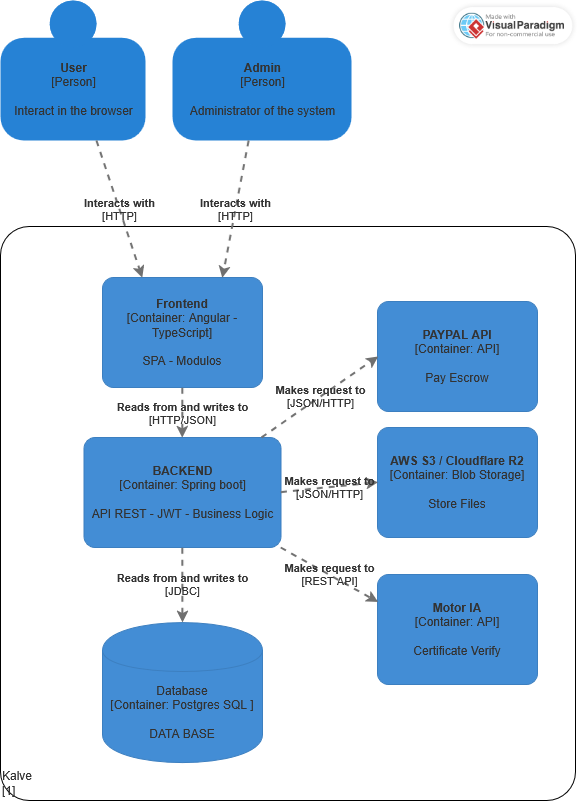
\includegraphics[width=0.85\textwidth]{c4-nivel2-contenedores.png}
\caption{Diagrama C4 Nivel 2 --- Contenedores de Artisync. Fuente:
\texttt{docs/diagramas/c4-nivel2-contenedores.png}.}
\label{fig:c4-nivel2}
\end{figure}

\textbf{Nota de honestidad sobre versiones documentadas vs. reales:} los
diagramas C4 (y \texttt{ADR-001}) documentan la pila como ``Java~25 +
Spring Boot~4.0.1'' y ``PostgreSQL~18/Angular~22'' en su versión
original. La pila \textbf{realmente construida y desplegada}, verificada
contra \texttt{pom.xml}, los \texttt{Dockerfile} y
\texttt{docker-compose.yml} a la fecha de este documento, es: \textbf{Java
21~LTS} (target de bytecode) \textbf{+ Spring Boot~4.1.0}, compilado en
contenedor \texttt{maven:3.9-eclipse-temurin-21} y ejecutado en
\texttt{eclipse-temurin:21-jre-alpine}; \textbf{Angular \^{}22.0.0} sobre
\texttt{node:24-alpine}; \textbf{PostgreSQL~16} (\texttt{postgres:16},
anclado por digest \texttt{sha256}) y \textbf{Redis~7}
(\texttt{redis:7-alpine}, igualmente anclado). La documentación
arquitectónica no se actualizó en cascada cuando el equipo fijó las
versiones finales --- ver \texttt{docs/entorno/versions.txt} para la
versión verificada y autoritativa, que este capítulo usa como fuente en
vez de repetir la cifra desactualizada de los diagramas.

\subsection{Nivel 3 --- Componentes (backend)}

El backend se organiza en siete módulos funcionales por dominio
(\texttt{seguridad}, \texttt{perfil}, \texttt{catalogo},
\texttt{pedido}/flujo de trabajo, \texttt{legal}, \texttt{comunicacion},
\texttt{social}), cada uno con sus capas
\texttt{entity}/\texttt{dto}/\texttt{repository}/\texttt{service}/\texttt{controller}.
Detalle completo: \texttt{docs/diagramas/C4\_Nivel3\_Componentes\_Backend.md}.

\section{Resumen de los siete registros de decisión de arquitectura (ADR)}

Los siete ADR siguen la plantilla de Nygard~\cite{NYGARD2011}:

Como se detalla en la Tabla~\\ref{tab:adrs}, 
Como se detalla en la Tabla~\\ref{tab:iso25010}, 
\begin{table}[H]
\centering
\caption{Resumen de los siete ADR de Artisync}
\label{tab:adrs}
\begin{tabular}{@{}p{1.4cm}p{3.4cm}p{9.4cm}@{}}
\toprule
\textbf{ADR} & \textbf{Título} & \textbf{Decisión resumida} \\
\midrule
ADR-001 & Selección de la pila tecnológica principal & Java/Spring Boot en
  el backend (mayor throughput, seguridad/persistencia integradas),
  Angular/TypeScript en el frontend, PostgreSQL como motor relacional,
  Redis como caché, Docker Compose como orquestador --- ver nota de
  versiones \S6.1. \\
ADR-002 & Esquema de autenticación y control de acceso & JWT (HS256)
  devuelto en el cuerpo de la respuesta para el access token (no en
  cookie); refresh token y ticket pre-auth de 2FA en cookies
  \texttt{HttpOnly + SameSite=Strict}; blacklist de JTI en Redis; bcrypt
  factor 12; RBAC vía Spring Security. Revisado en agosto 2026 tras
  corregir una afirmación incorrecta de una versión anterior del ADR (ver
  texto completo). \\
ADR-003 & Selección del gestor de base de datos & PostgreSQL~16 sobre
  MySQL/MariaDB y MongoDB, por ACID completo, tipos \texttt{DECIMAL}
  precisos para montos financieros, y soporte maduro de PL/pgSQL para la
  estrategia híbrida de acceso a datos (ADR-006). \\
ADR-004 & Estrategia de caché & Redis~7 para caché de catálogo (TTL
  configurable), blacklist de JTI, cuotas de rate limiting y tickets
  pre-auth 2FA, sobre caché en memoria de la JVM, por ser compartido entre
  réplicas si el backend escala horizontalmente. \\
ADR-005 & Estrategia de despliegue y reproducibilidad & Docker Compose con
  imágenes ancladas por digest \texttt{sha256} + \texttt{Makefile} de un
  solo comando, sobre despliegue manual o imágenes por tag variable, para
  máxima reproducibilidad (badge ACM \emph{Artifacts Evaluated ---
  Reusable}). Las tres acciones pendientes de la Tercera Entrega
  (Frontend/ ausente, digests por tag, Makefile inexistente) están
  resueltas y verificadas a la fecha de la Entrega Final. \\
ADR-006 & Estrategia híbrida de acceso a datos & CRUD elementales vía
  JPA/Spring Data; operaciones con joins, agregaciones, reportes,
  actualizaciones masivas o validaciones cruzadas vía
  procedimientos/funciones PL/pgSQL versionados en \texttt{db/procs/},
  invocados exclusivamente mediante JPA~2.1. Ampliado el 16 de agosto de
  2026 con 7 rutinas nuevas conectadas end-to-end (ver
  Capítulo~\ref{cap:implementacion}). \\
ADR-007 & Almacenamiento de archivos en la nube & Azure Blob Storage como
  único destino en la nube (sobre un esquema híbrido Cloudinary+Azure Blob
  o mantener el volumen local), detrás de la interfaz
  \texttt{AlmacenamientoDocumentos}, seleccionable por configuración
  (\texttt{documentos.proveedor}). \\
\bottomrule
\end{tabular}
\end{table}

Texto completo de cada ADR, con contexto, opciones descartadas y
consecuencias, en \texttt{docs/adr/}.

\section{Atributos de calidad (ISO/IEC 25010) --- prioridad, escenario y estrategia}

\begin{table}[H]
\centering
\caption{Atributos de calidad ISO/IEC~25010~\cite{ISO25010} priorizados}
\label{tab:iso25010}
\begin{tabular}{@{}p{3.0cm}p{1.6cm}p{4.0cm}p{5.6cm}@{}}
\toprule
\textbf{Característica ISO~25010} & \textbf{Prioridad} & \textbf{Escenario} & \textbf{Estrategia aplicada} \\
\midrule
Eficiencia de desempeño (rendimiento) & Alta & Listado de catálogo bajo 50
  usuarios concurrentes & Caché Redis con TTL (ADR-004); índices en
  columnas de filtro; medido con k6 (Capítulo~\ref{cap:evaluacion-resultados}) \\
Seguridad & Alta & Acceso no autorizado a rutas protegidas, inyección
  SQL, credenciales en tránsito & RBAC + JWT (ADR-002);
  procedimientos/consultas parametrizadas (ADR-006); rate limiting;
  auditoría estática y dinámica automatizada
  (Capítulo~\ref{cap:evaluacion-resultados}) \\
Fiabilidad & Alta & Caída de un contenedor dependiente (Redis, Postgres) &
  \texttt{healthcheck} de Docker Compose con
  \texttt{depends\_on: condition: service\_healthy};
  \texttt{/actuator/health} expone estado por componente \\
Usabilidad & Media & Usuario nuevo completa el flujo de contratación sin
  asistencia & Formularios dinámicos, flujo de contratación acotado (SRS
  \texttt{REQ-NF-008}); medido con SUS
  (Capítulo~\ref{cap:evaluacion-resultados}) \\
Mantenibilidad & Media & Incorporar un nuevo procedimiento almacenado sin
  tocar el código Java existente & Módulos desacoplados por dominio
  (Nivel~3 C4); \texttt{scripts/sync-procs.sh} mantiene sincronizada la
  migración repetible \\
Portabilidad & Media & Desplegar en un proveedor cloud distinto al usado
  en desarrollo & Configuración externalizada (\texttt{.env}),
  \texttt{documentos.proveedor} seleccionable (ADR-007), imágenes ancladas
  por digest (ADR-005) \\
Compatibilidad & Baja & Integración con PayPal Orders v2 y servicio
  externo de IA & Contratos de API versionados, adaptadores dedicados por
  integración \\
\bottomrule
\end{tabular}
\end{table}

\section{Modelo de datos}

El esquema relacional completo se versiona con Flyway; el modelo
entidad-relación se mantiene en \texttt{docs/diagramas/Entidad\_Relacion.png}
(ver nota de conformidad de nombres de tablas en \texttt{ADR-003}).

\begin{figure}[H]
\centering
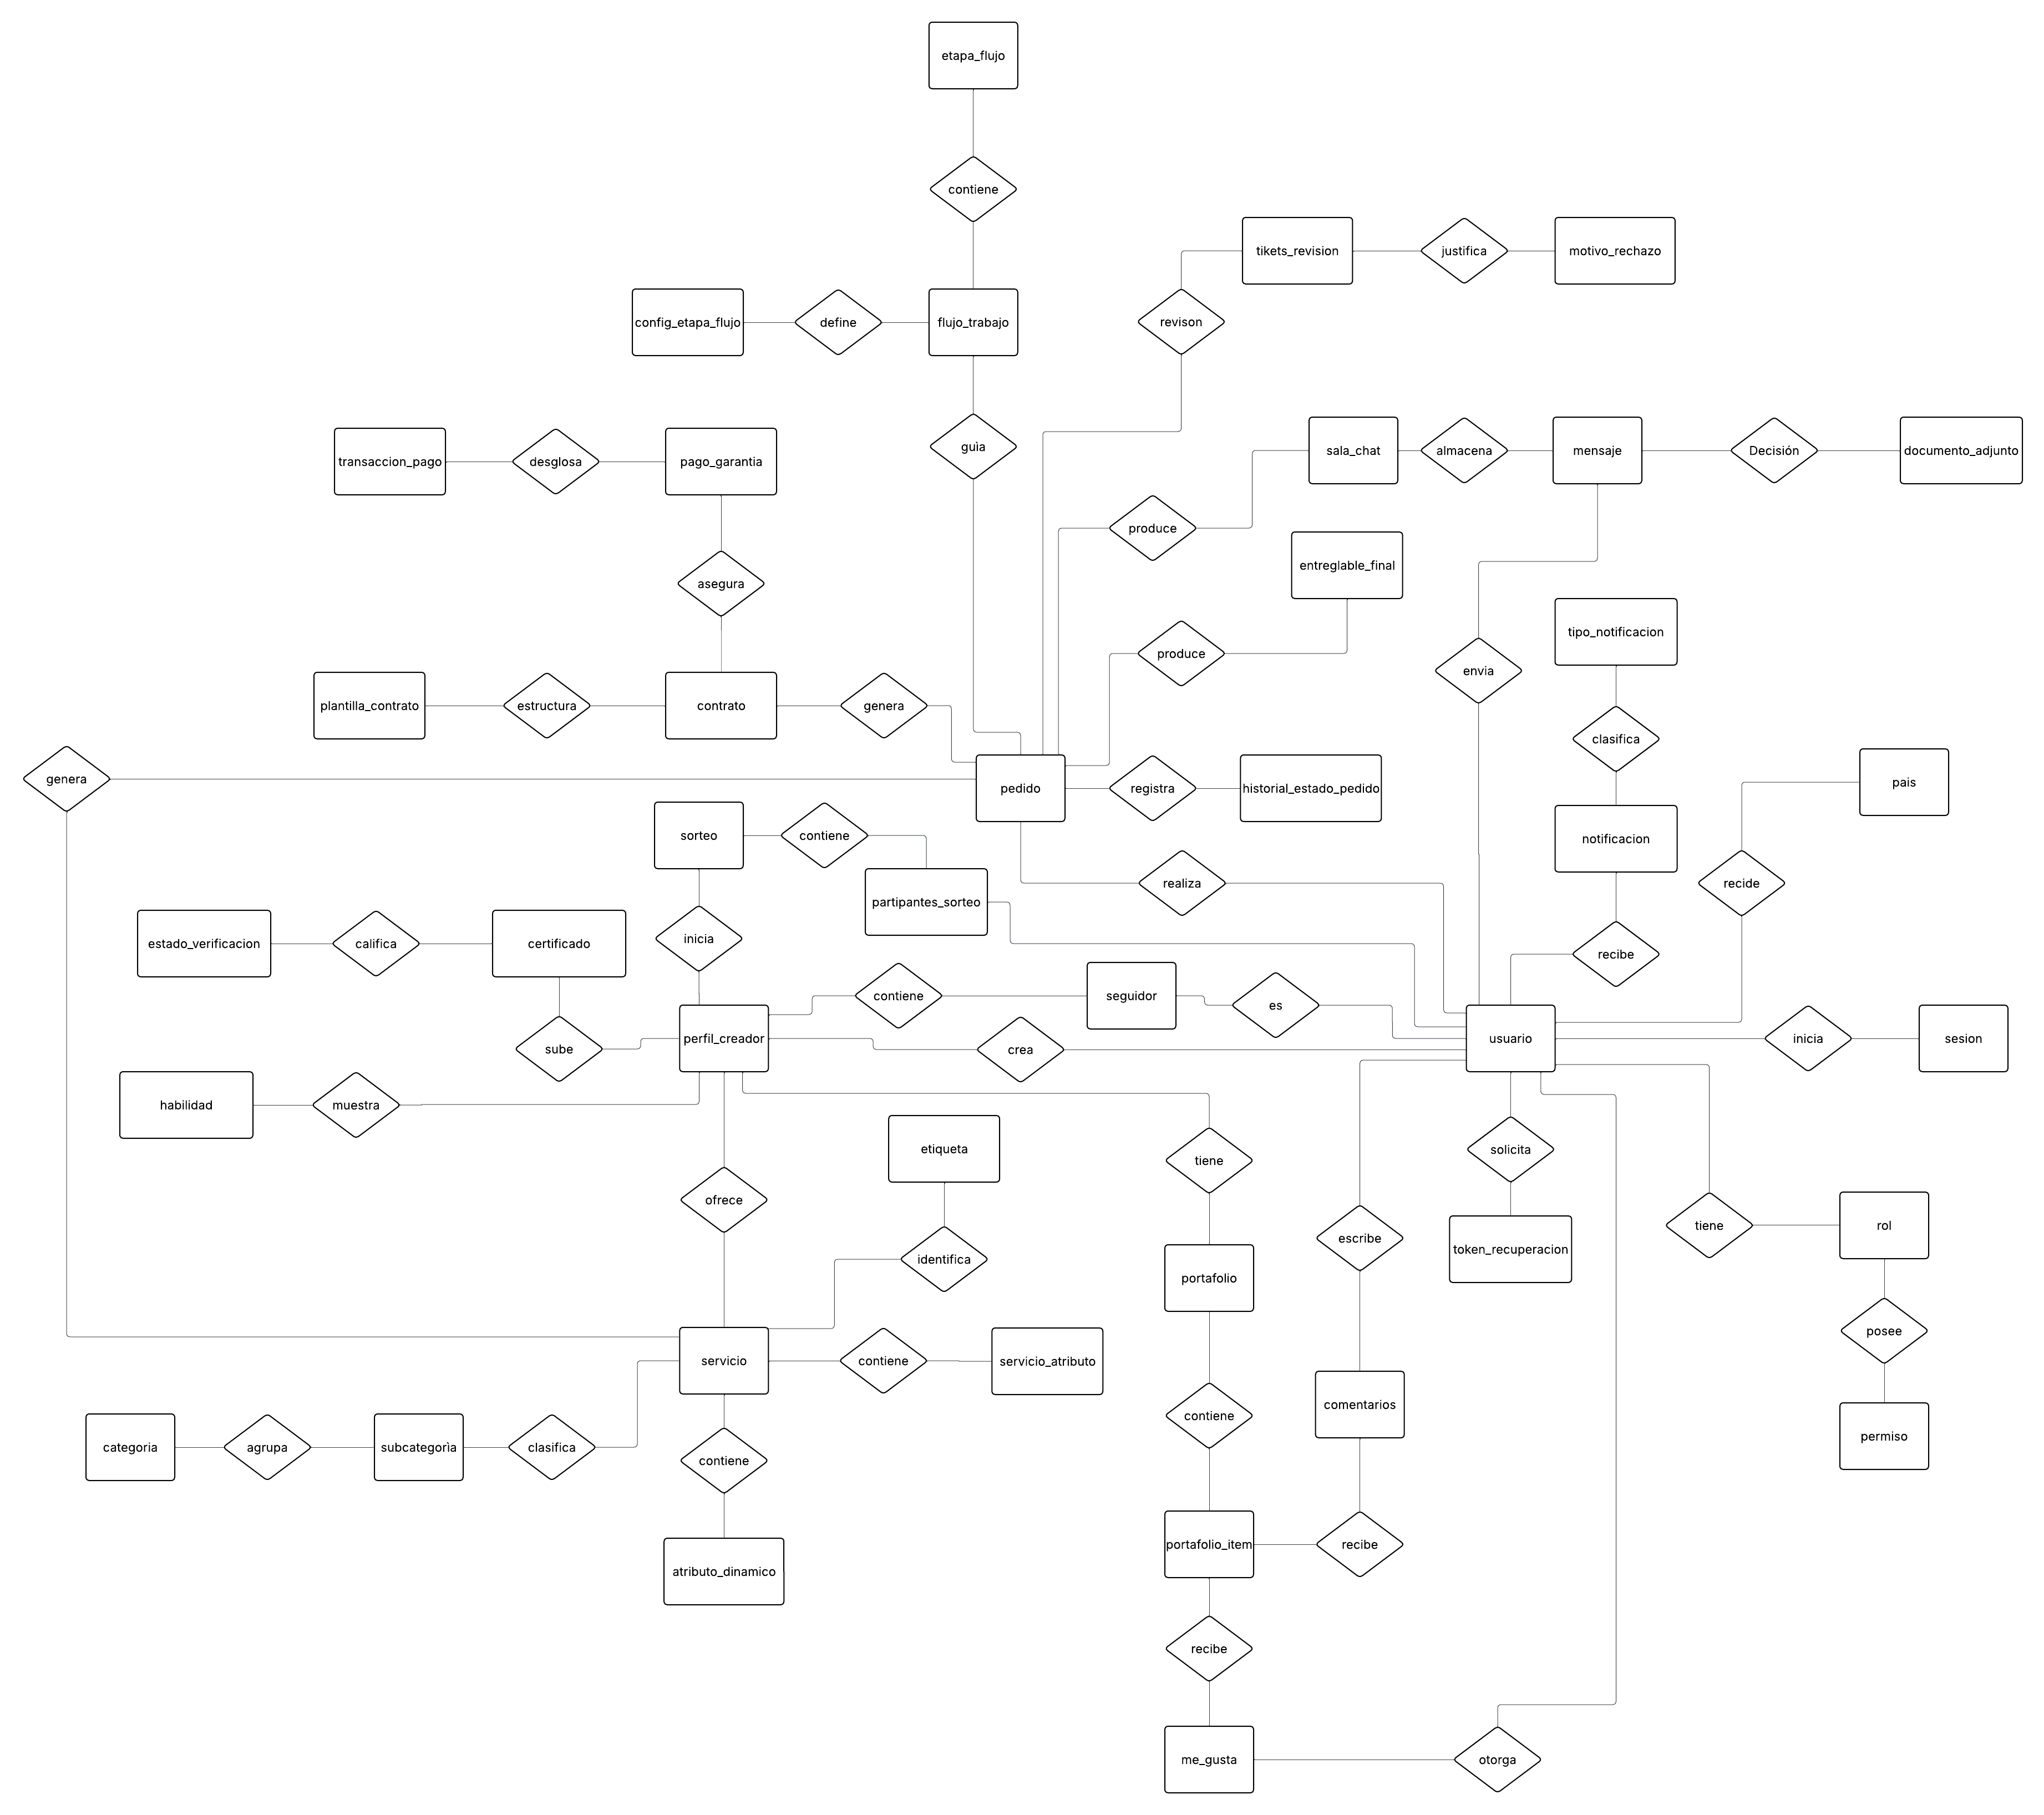
\includegraphics[width=0.95\textwidth]{Entidad_Relacion.png}
\caption{Modelo entidad-relación de Artisync. Fuente:
\texttt{docs/diagramas/Entidad\_Relacion.png}.}
\label{fig:mer}
\end{figure}

\section{Matriz de trazabilidad}

La matriz completa (37 filas: requisito $\to$ historia de usuario $\to$
caso de uso $\to$ módulo de código $\to$ endpoint $\to$ prueba
automatizada $\to$ \textbf{tipo de acceso} $\to$ evidencia empírica
$\to$ estado) está en \texttt{docs/trazabilidad/matriz.csv}, validada
automáticamente en CI por \texttt{scripts/validate-traceability.sh}. La
columna \texttt{tipo\_acceso} distingue \texttt{CRUD-ORM} de \texttt{SP}
(procedimiento almacenado): a la fecha de este documento, 8 filas están
marcadas \texttt{SP} (correspondientes a los 7 requisitos que ya invocan
una de las rutinas conectadas end-to-end, ver
Capítulo~\ref{cap:implementacion}), el resto \texttt{CRUD-ORM}.

% 07-implementacion.tex — Fuente: docs/informe-final/07-implementacion.md

\chapter{Implementación}
\label{cap:implementacion}

No se transcriben archivos completos; se remite al repositorio para el
detalle. Este capítulo ilustra con listados pequeños y significativos las
decisiones críticas de código.

\section{Manejo de errores globales (RFC 7807 Problem Details)}

Todos los errores de la API se serializan como \texttt{ProblemDetail}
(RFC~7807), en vez de estructuras JSON ad-hoc distintas por controlador, como se puede observar en el Listado~\ref{lst:manejador-excepciones}.

\begin{lstlisting}[language=Java,caption={Manejador global de excepciones (RFC 7807 ProblemDetail). Fuente: \texttt{artisync/\allowbreak Backend/\allowbreak src/\allowbreak main/\allowbreak java/\allowbreak .../\allowbreak exception/\allowbreak ManejadorGlobalExcepciones.java}},label=lst:manejador-excepciones]
@Slf4j
@RestControllerAdvice
public class ManejadorGlobalExcepciones {

    private static final String BASE_TIPO = "https://artisync.dev/errors/";

    @ExceptionHandler(AccessDeniedException.class)
    public ResponseEntity<ProblemDetail> manejarAccesoDenegado(AccessDeniedException ex) {
        ProblemDetail problema = ProblemDetail.forStatus(HttpStatus.FORBIDDEN);
        problema.setType(URI.create(BASE_TIPO + "acceso-denegado"));
        problema.setTitle("Acceso denegado");
        // ... (continua con los demas @ExceptionHandler: validacion, JWT, 404, etc.)
    }
}
\end{lstlisting}

Esta decisión centraliza el formato de error para las 1230 pruebas del
backend y para el interceptor HTTP del frontend Angular, evitando el
manejo de errores ad-hoc por controlador.

\section{Esquema de caching}

El listado de catálogo (endpoint de mayor frecuencia de lectura,
\texttt{REQ-NF-004}) usa Spring Cache sobre Redis (\texttt{ADR-004}), con
invalidación automática (\texttt{@CacheEvict}) al crear/editar/eliminar
un servicio, tal como se muestra en el Listado~\ref{lst:cache-catalogo}:

\begin{lstlisting}[language=Java,caption={Caché del listado de catálogo (Spring Cache + Redis). Fuente: \texttt{artisync/\allowbreak Backend/\allowbreak src/\allowbreak main/\allowbreak java/\allowbreak .../\allowbreak service/\allowbreak catalogo/\allowbreak impl/\allowbreak ServicioCatalogoServicioImpl.java}},label=lst:cache-catalogo]
@Override
@Transactional(readOnly = true)
@Cacheable(cacheNames = "catalogo")
public Page<RespuestaServicioResumido> buscarCatalogoServicios(
        Long categoriaId, Long subcategoriaId, BigDecimal precioMin, BigDecimal precioMax,
        List<Long> etiquetaIds, String textoBusqueda, String sortParam, int page, int size) {
    // ... construye la Specification dinamica y ejecuta la consulta paginada
}
\end{lstlisting}

La clave de caché de Spring se compone de todos los parámetros del método
--- una limitación de diseño relevante para la interpretación de los
resultados de rendimiento del Capítulo~\ref{cap:evaluacion-resultados}
(ver \texttt{docs/mediciones/perf/REPORTE-PERF.md}, advertencia
metodológica sobre el escenario ``frío'').

\section{Mecanismo de seguridad: JWT + rate limiting}

La autenticación es \emph{stateless} (JWT~\cite{JWT2015}, \texttt{ADR-002});
las rutas de autenticación aplican rate limiting por IP real (resuelta
vía \texttt{server.forward-headers-strategy=native}, no
\texttt{getRemoteAddr()} directo) y por cuenta, con respuesta \texttt{429}
en formato \texttt{ProblemDetail} --- ver \texttt{AuthRateLimitFilter} e
\texttt{IntentosAutenticacionService}, corrección de la observación
\texttt{OBS-AUTO-05} documentada en \texttt{docs/observaciones/OBSERVACIONES.md}.
El diagrama de la Figura~\ref{fig:secuencia-jwt} ilustra la secuencia.

\begin{figure}[H]
\centering
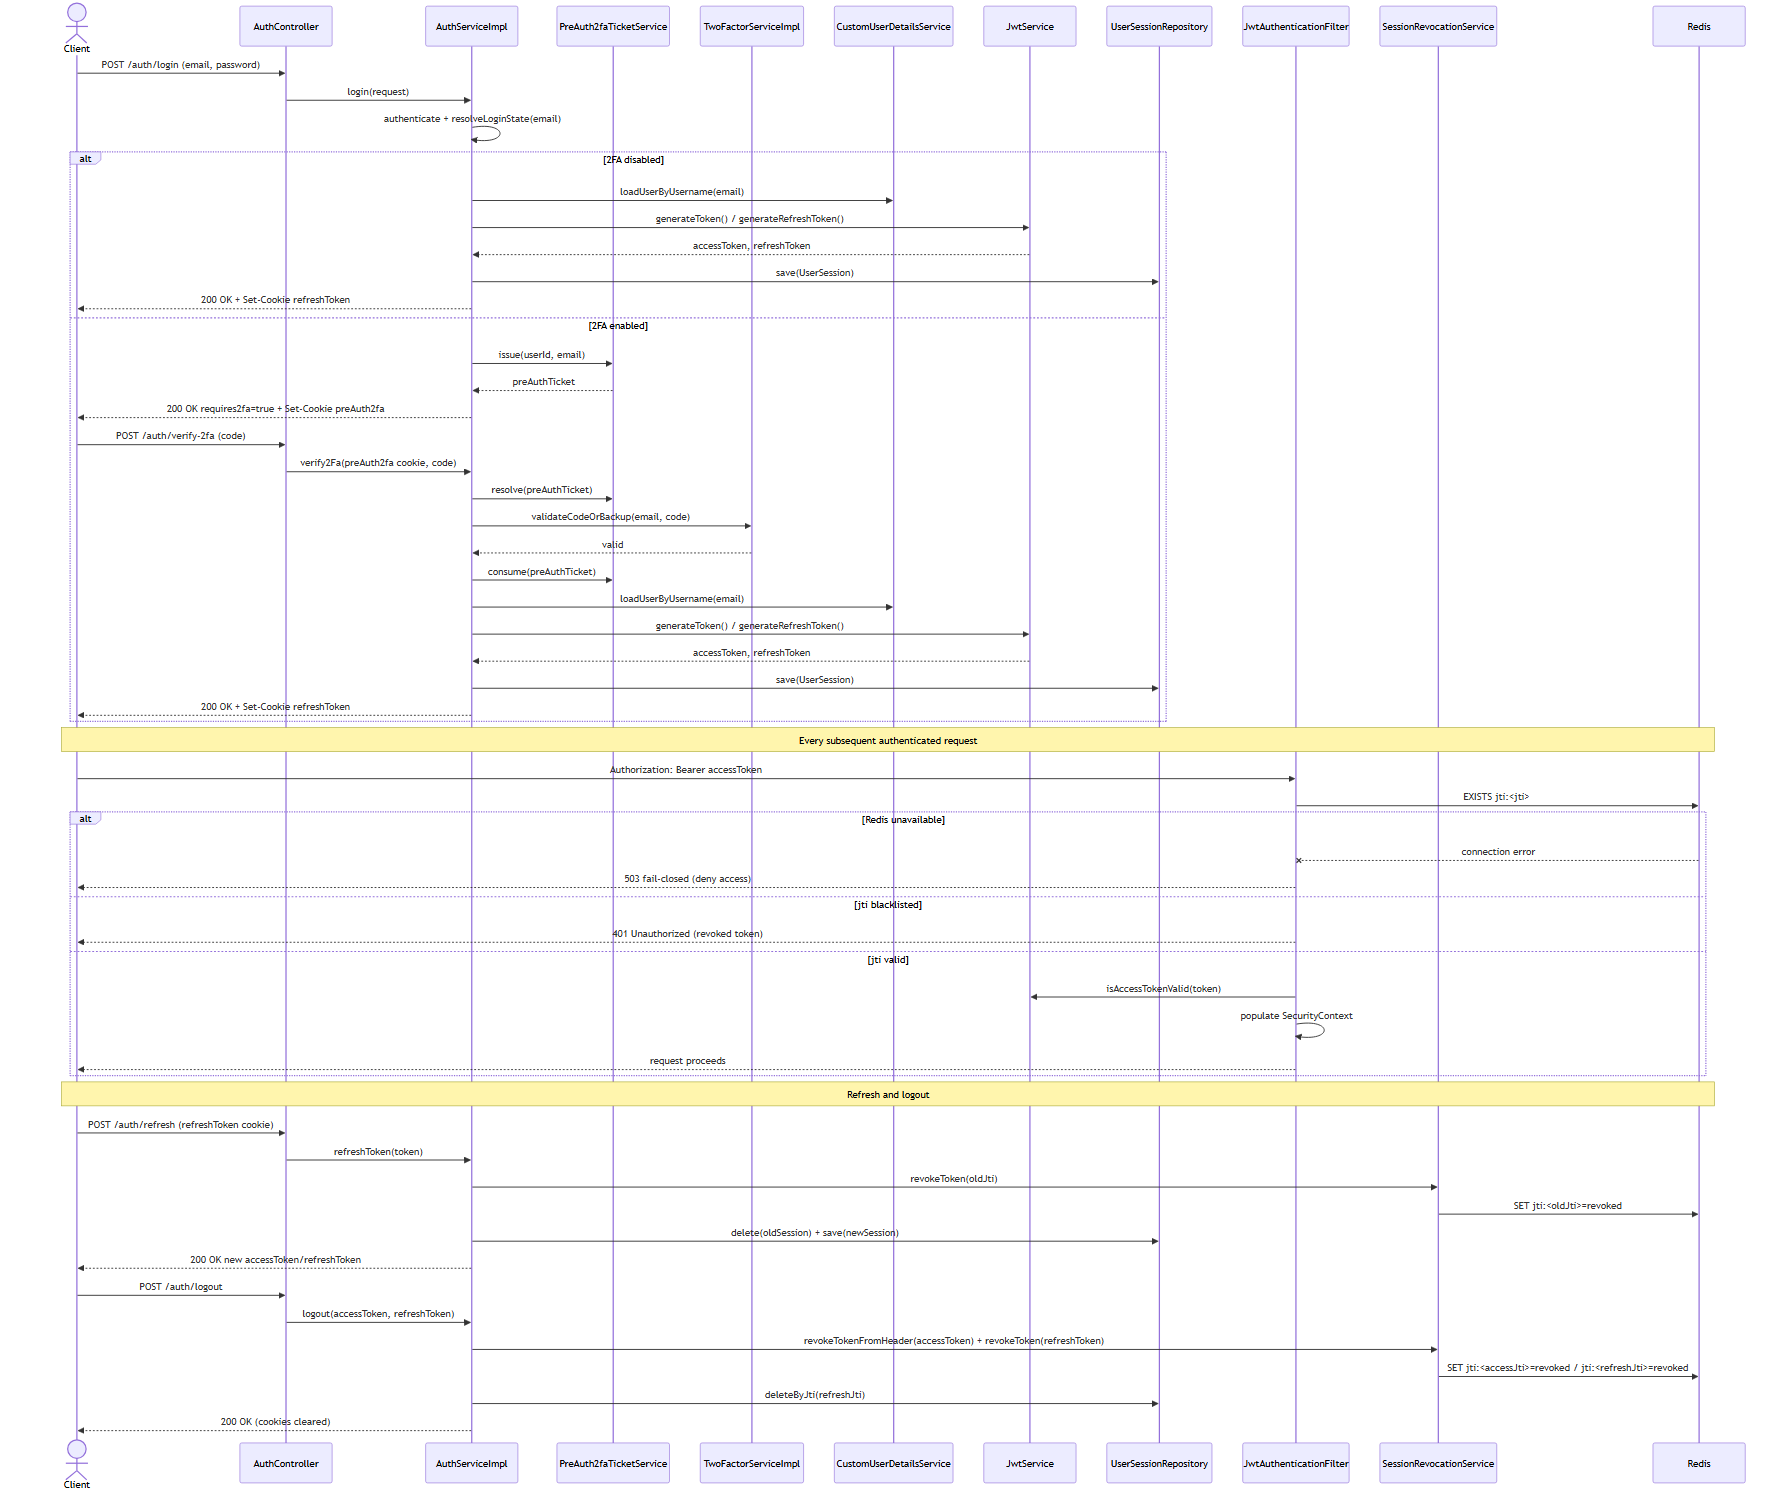
\includegraphics[width=0.85\textwidth]{secuencia_login_jwt.png}
\caption{Diagrama de secuencia del flujo de autenticación JWT. Fuente:
\texttt{docs/diagramas/secuencia\_login\_jwt.png}.}
\label{fig:secuencia-jwt}
\end{figure}

\section{Estrategia híbrida de acceso a datos: procedimiento almacenado representativo}
\label{sec:acceso-datos-hibrido}

Esta subsección ilustra el contrato completo entre un procedimiento
versionado en \texttt{db/procs/} y el método de repositorio Spring Data
que lo invoca, siguiendo la especificación JPA~2.1 (\texttt{ADR-006},
Capítulo~\ref{cap:diseno-arquitectura}~\S6.2).
El Listado~\ref{lst:sp-registrar-decision} presenta la definición SQL, mientras que el Listado~\ref{lst:repo-registrar-decision} detalla su invocación formal con la anotación \texttt{@Procedure}.

\begin{lstlisting}[language=SQL,caption={\texttt{sp\_registrar\_decision\_verificacion} (categoría: validaciones cruzadas). Fuente: \texttt{artisync/\allowbreak Backend/\allowbreak src/\allowbreak main/\allowbreak resources/\allowbreak db/\allowbreak migration/\allowbreak V7\_\_verificacion\_asistida\_ia.sql}},label=lst:sp-registrar-decision]
CREATE OR REPLACE PROCEDURE sp_registrar_decision_verificacion(
    p_id_certificado BIGINT,
    p_id_estado BIGINT,
    p_id_moderador BIGINT,
    p_nota TEXT
)
LANGUAGE plpgsql
AS $$
BEGIN
    UPDATE certificados_ia 
    SET id_estado = p_id_estado, id_moderador = p_id_moderador, nota = p_nota, fecha_analisis = NOW()
    WHERE id_certificado = p_id_certificado;
END;
$$;
\end{lstlisting}

\begin{lstlisting}[language=Java,caption={Método de repositorio que invoca \texttt{sp\_registrar\_decision\_verificacion}. Fuente: \texttt{artisync/\allowbreak Backend/\allowbreak src/\allowbreak main/\allowbreak java/\allowbreak .../\allowbreak repository/\allowbreak profile/\allowbreak AiCertificateRepository.java}},label=lst:repo-registrar-decision]
    @Procedure(procedureName = "sp_registrar_decision_verificacion")
    void registrarDecision(
            @Param("p_id_certificado") Long idCertificado,
            @Param("p_id_estado") Long idEstado,
            @Param("p_id_moderador") Long idModerador,
            @Param("p_nota") String nota);
\end{lstlisting}

\subsection{Conformidad lograda}

La invocación utiliza los mecanismos formales de la
especificación JPA~2.1 mediante la anotación \texttt{@Procedure} sobre el método del
repositorio Spring Data, asegurando una conexión segura y \textbf{sin
concatenación de cadenas} (evitando así la inyección SQL, conforme al
análisis de Gould~\cite{GOULD2004} y Halfond~\cite{HALFOND2005}). Este
esquema resuelve plenamente los requerimientos de seguridad y diseño arquitectónico (ver Sección~\ref{sec:acceso-datos-hibrido}).

\subsection{Resolución aplicada: rutinas con retorno escalar}

\texttt{@Procedure} se aplica de forma sistemática cuando el método Java es
\texttt{void} y la rutina no declara ningún parámetro \texttt{OUT}/\texttt{INOUT}: además de
\texttt{sp\_registrar\_decision\_verificacion} (Listado~\ref{lst:repo-registrar-decision}), es el
caso de \texttt{sp\_restablecer\_contrasena} y \texttt{sp\_cambiar\_contrasena}, migradas y
verificadas contra el stack real (revisión técnica 2026-09-05).

Para las rutinas que necesitan devolver un valor escalar --- por ejemplo
\texttt{fn\_registrar\_usuario}, \texttt{fn\_resolver\_estado\_login} o
\texttt{fn\_permisos\_efectivos\_usuario} (esta última se ejecuta en cada inicio de sesión) --- se
investigó en tres rondas independientes (2026-09-05, 2026-09-14 y una verificación adicional la
misma noche) si podían invocarse con \texttt{@Procedure}/\texttt{@NamedStoredProcedureQuery}. Las
tres coincidieron en el mismo resultado: en cuanto un método declara un tipo de retorno distinto de
\texttt{void}, Hibernate~7.4.1 serializa \emph{todos} los parámetros --- incluido el propio valor de
retorno --- con la sintaxis de argumento nombrado de PostgreSQL dentro del \emph{JDBC escape}
\texttt{\{call ...\}}, que PostgreSQL no puede interpretar ahí
(\texttt{ERROR: syntax error at or near "=>"}). Se confirmó que ni los parámetros puramente
posicionales evitan el defecto (Spring Boot compila con \texttt{-parameters} y Hibernate obtiene el
nombre por reflexión de todos modos), ni una versión de parche posterior de Hibernate
(\texttt{7.4.5.Final}, probada explícitamente contra Postgres real y revertida sin dejar rastro) lo
corrige. La única vía que evita el defecto --- la API nativa imperativa de Hibernate
(\texttt{Session.createStoredProcedureCall} + \texttt{markAsFunctionCall}) --- es estructuralmente
inalcanzable desde cualquier anotación JPA declarativa: exigiría abandonar
\texttt{@Procedure}/\texttt{@NamedStoredProcedureQuery} por completo e implementar cada método a
mano. Un commit del 4 de septiembre de 2026 que migró estas rutinas a \texttt{@Procedure} sin
conocer aún esta restricción rompió el inicio de sesión en producción; se revirtió y motivó esta
investigación. El detalle completo, con la orden y la salida de cada prueba contra Postgres real,
está en \texttt{docs/basedatos/CATALOGO-SP.md} (\S14).

\textbf{Resolución (14-sep-2026, cierre del Punto~P6 de la guía del examen suspenso):} la guía
exige, literalmente, \emph{cero apariciones de \texttt{nativeQuery=true} para invocar
procedimientos almacenados} --- no exige la anotación \texttt{@Procedure} en sí. Puesto que ninguna
vía dentro de JPA/Hibernate evita el defecto sin renunciar a una anotación declarativa, la solución
fue salir de JPA/Hibernate por completo para estas 23 rutinas: se sustituyó
\texttt{@Query(nativeQuery = true)} por \texttt{NamedParameterJdbcTemplate}
(\texttt{org.springframework.jdbc.core.namedparam}), que construye la sentencia como texto
(\texttt{SELECT fn\_x(:parametro)}) y la ejecuta por JDBC puro, sin instanciar nunca un
\texttt{Session}/\texttt{EntityManager} de Hibernate --- y por tanto sin pasar por las clases donde
se origina el defecto (\texttt{PostgreSQLCallableStatementSupport},
\texttt{NamedCallableQueryMementoImpl}). El patrón aplicado es consistente con código ya existente
en el proyecto (\texttt{ContractRepositoryCustom}/\texttt{ContractRepositoryImpl}, que ya resolvía
consultas dinámicas complejas por fuera de \texttt{@Query}): cada repositorio afectado gana una
interfaz \texttt{XxxRepositoryCustom} y una clase \texttt{XxxRepositoryImpl} que la implementa
inyectando \texttt{NamedParameterJdbcTemplate}; para quien invoca el repositorio no cambia nada,
Spring Data fusiona ambas interfaces por convención de nombre.

Se verificó que este cambio no reproduce el incidente de producción del 4 de septiembre de 2026 que
motivó originalmente la excepción: suite completa de pruebas (1448/1448), 31 pruebas de integración
contra Postgres real, y login, registro, recuperación de contraseña y gestión de roles/países
probados a mano contra el backend con Postgres real, incluida la captura del \texttt{Set-Cookie}
real del login.

De paso se revisaron también los dos \texttt{PROCEDURE} de purga
(\texttt{sp\_purgar\_notificaciones}, \texttt{sp\_purgar\_datos\_seguridad}, invocados hoy con
\texttt{JdbcTemplate.update("CALL ...")} desde \texttt{NotificationPurgeScheduler} y
\texttt{SecurityPurgeScheduler}): son \texttt{void}, solo parámetros \texttt{IN}, exactamente el
patrón que sí funciona con \texttt{@Procedure}, pero ambos ejecutan \texttt{COMMIT} explícito por
lote dentro del propio \texttt{PROCEDURE} (para no sostener una transacción larga que bloquee
\texttt{VACUUM}), lo que exige que la conexión no tenga ya una transacción abierta por Spring
(\texttt{Propagation.NOT\_SUPPORTED} está declarado como obligatorio en ambos \textit{schedulers},
no cosmético) --- Postgres falla con \texttt{2D000 invalid\_transaction\_termination} si el
\texttt{CALL} ocurre dentro de una transacción ya iniciada. Se mantienen en \texttt{JdbcTemplate}
directo --- ya usaban este mismo mecanismo antes de la migración de las otras 23 rutinas --- no por
descuido sino por esta restricción de manejo de transacciones, independiente del defecto de
Hibernate.

De las 28 rutinas activas (26 de \texttt{db/procs/} más 2 de verificación asistida por IA), el
reparto exacto por mecanismo de invocación --- verificable de forma reproducible con
\texttt{python scripts/auditoria-rubrica.py p6}, que descuenta las menciones dentro de comentarios
Javadoc --- es: \textbf{3} vía \texttt{@Procedure} (método \texttt{void}, sin parámetros
\texttt{OUT}/\texttt{INOUT}), \textbf{0} vía \texttt{@NamedStoredProcedureQuery}, \textbf{0} vía
\texttt{@Query(nativeQuery = true)} y \textbf{25} vía \texttt{NamedParameterJdbcTemplate} (las 23
migradas en esta resolución más las 2 rutinas de purga, que ya usaban este mecanismo desde antes por
la restricción de transacciones descrita arriba). El mecanismo de acceso a datos, en conjunto, sigue
siendo \emph{híbrido y documentado por diseño} (ADR-006), no accidental ni pendiente de resolución.

% 08-evaluacion-resultados.tex — Fuente: docs/informe-final/08-evaluacion-resultados.md

\chapter{Evaluación empírica y resultados}
\label{cap:evaluacion-resultados}

Cada bloque se reporta con: (i) pregunta de investigación asociada, (ii)
métrica, (iii) datos crudos y su ubicación, (iv) estadística descriptiva,
y (v) interpretación textual.

\section{Rendimiento (k6) --- RQ1}

\textbf{Métrica:} percentiles de latencia (\texttt{http\_req\_duration}) y
tasa de error HTTP $\geq$500 sobre
\texttt{GET /api/v1/catalogo?page=0\&size=20}, 50~VUs, 30~s, 3 corridas
por escenario. \textbf{Datos crudos:}
\texttt{docs/mediciones/perf/k6-run\{1,2,3\}.json} (caliente),
\texttt{k6-cold-run\{1,2,3\}.json} (frío); consolas en
\texttt{k6-console-run*.txt}.

\begin{table}[H]
\centering
\caption{Resultados de la prueba de carga k6 por escenario}
\label{tab:k6}
\resizebox{\textwidth}{!}{%
\begin{tabular}{@{}lrrrrrlr@{}}
\toprule
\textbf{Escenario} & \textbf{n} & \textbf{Media (ms)} & \textbf{Mediana (ms)} & \textbf{DT (ms)} & \textbf{IC 95\,\% (ms)} & \textbf{p50/p90/p95/p99 (ms)} & \textbf{Error $\geq$500} \\
\midrule
Caliente & 4500 & 21.38 & 13.01 & 32.71 & [20.42, 22.33] & 13.01 / 31.75 / \textbf{50.17} / 205.60 & 0.00\,\% \\
Frío     & 4500 & 13.62 &  9.04 & 14.52 & [13.20, 14.05] &  9.04 / 22.39 / \textbf{39.14} /  89.98 & 0.00\,\% \\
\bottomrule
\end{tabular}}
\end{table}

\textbf{Umbral:} p95 $\leq$200~ms caliente (\textbf{cumple}, 50.17~ms),
p95 $\leq$500~ms frío (\textbf{cumple}, 39.14~ms). Throughput
$\approx$48.5--49.0~req/s por corrida.

\textbf{Interpretación:} ambos escenarios cumplen holgadamente sus
umbrales respectivos. El hallazgo más relevante no es el cumplimiento en
sí, sino que el escenario ``frío'' resultó \textbf{más rápido} que el
``caliente'' --- contraintuitivo, y documentado con honestidad
metodológica en \texttt{docs/mediciones/perf/REPORTE-PERF.md}: el script
de carga golpea siempre la misma combinación de parámetros de consulta,
por lo que la clave de caché de Spring (\texttt{@Cacheable},
Capítulo~\ref{cap:implementacion}~\S7.2) se puebla con la primera
petición en ambos escenarios --- de las 1500 iteraciones por corrida, como
mucho una es un \emph{miss} real contra PostgreSQL. La diferencia de
medias observada (21.38~ms vs. 13.62~ms) es ruido de ejecución (JIT/GC de
la JVM, carga del contenedor), no un efecto real de caché frío vs.
caliente. \textbf{No se ejecutó} el test inferencial (Wilcoxon) ni el
tamaño de efecto que exige el Bloque~C de la guía para esta comparación
--- protocolo recomendado por Arcuri y Briand~\cite{ARCURI2011},
declarado como brecha en el Capítulo~\ref{cap:materiales-metodos}~\S5.6 y
retomado como amenaza a la validez en el Capítulo~\ref{cap:validez}.

\section{Seguridad (OWASP + ZAP + análisis estático) --- RQ1, RQ2}

\textbf{Métrica:} estado (aprobado/hallazgo) de 6 controles
OWASP~\cite{OWASP2021} evidenciados manualmente, más el resultado
agregado del escaneo automatizado ZAP baseline y del análisis estático
SpotBugs + find-sec-bugs~\cite{HALFOND2005,GOULD2004}. \textbf{Datos
crudos:} \texttt{docs/mediciones/sec/owasp/*.txt}, \texttt{sec/zap/},
\texttt{sec/static-analysis/}.

\begin{table}[H]
\centering
\caption{Controles OWASP evidenciados manualmente}
\label{tab:owasp}
\begin{tabular}{@{}p{5.4cm}p{2.0cm}p{5.6cm}@{}}
\toprule
\textbf{Control OWASP} & \textbf{Estado} & \textbf{Evidencia} \\
\midrule
A01 --- Control de acceso roto & Aprobado & \texttt{sec/owasp/a01-control-acceso.txt} \\
A02 --- Fallas criptográficas (TLS) & Aprobado & \texttt{sec/owasp/a02-tls.txt} \\
A03 --- Inyección & Aprobado & \texttt{sec/owasp/a03-inyeccion.txt} \\
A05 --- Configuración de seguridad incorrecta & Aprobado & \texttt{sec/owasp/a05-cabeceras.txt} \\
A07 --- Fallas de identificación y autenticación & Aprobado & \texttt{sec/owasp/a07-rate-limit.txt} \\
A09 --- Fallas de registro y monitoreo & Aprobado & \texttt{sec/owasp/a09-logging.txt} \\
\bottomrule
\end{tabular}
\end{table}

A04, A06, A08, A10 quedan fuera de alcance declarado (no evaluados) --- ver
\texttt{docs/mediciones/sec/REPORTE-SEC.md}.

\textbf{ZAP baseline:} \texttt{FAIL-NEW: 0} $\cdot$ \texttt{WARN-NEW: 8}
(severidad media/baja, ninguno bloqueante) $\cdot$ \texttt{PASS: 59}.
Cumple el umbral de ``sin hallazgos altos''.

\textbf{Análisis estático (SpotBugs + find-sec-bugs):} \textbf{0
hallazgos} de inyección SQL
(\texttt{SQL\_NONCONSTANT\_STRING\_PASSED\_TO\_EXECUTE},
\texttt{SQL\_INJECTION\_JDBC} y variantes) sobre el bytecode del backend
completo --- consistente con el modelo de detección estático propuesto
originalmente por Gould, Su y Devanbu~\cite{GOULD2004}.

\textbf{Interpretación:} la combinación de evidencia manual reproducible
(6 controles) y escaneo automatizado (ZAP + análisis estático) da una
cobertura de seguridad consistente en ambas direcciones (top-down por
control OWASP, bottom-up por herramienta automatizada), sin
contradicciones entre ambas fuentes.

\section{Usabilidad (SUS) --- RQ1}

\textbf{Métrica:} puntaje System Usability Scale
(0--100)~\cite{BROOKE1996}, N=16 (umbral mínimo de la guía: N$\geq$15).
\textbf{Datos crudos:} \texttt{docs/mediciones/sus/sus-raw.csv}, perfil de
participantes en \texttt{perfil-participantes.csv}.

\begin{table}[H]
\centering
\caption{Resultados del cuestionario SUS}
\label{tab:sus}
\begin{tabular}{@{}lr@{}}
\toprule
\textbf{Métrica} & \textbf{Valor} \\
\midrule
n & 16 \\
Media & 76.88 \\
Mediana & 77.50 \\
DT & 14.48 \\
IC 95\,\% & [69.16, 84.59] \\
Interpretación (escala de Bangor~\cite{BANGOR2009}) & \textbf{B} \\
Umbral del proyecto ($>$68) & Supera \\
\bottomrule
\end{tabular}
\end{table}

\begin{figure}[H]
\centering
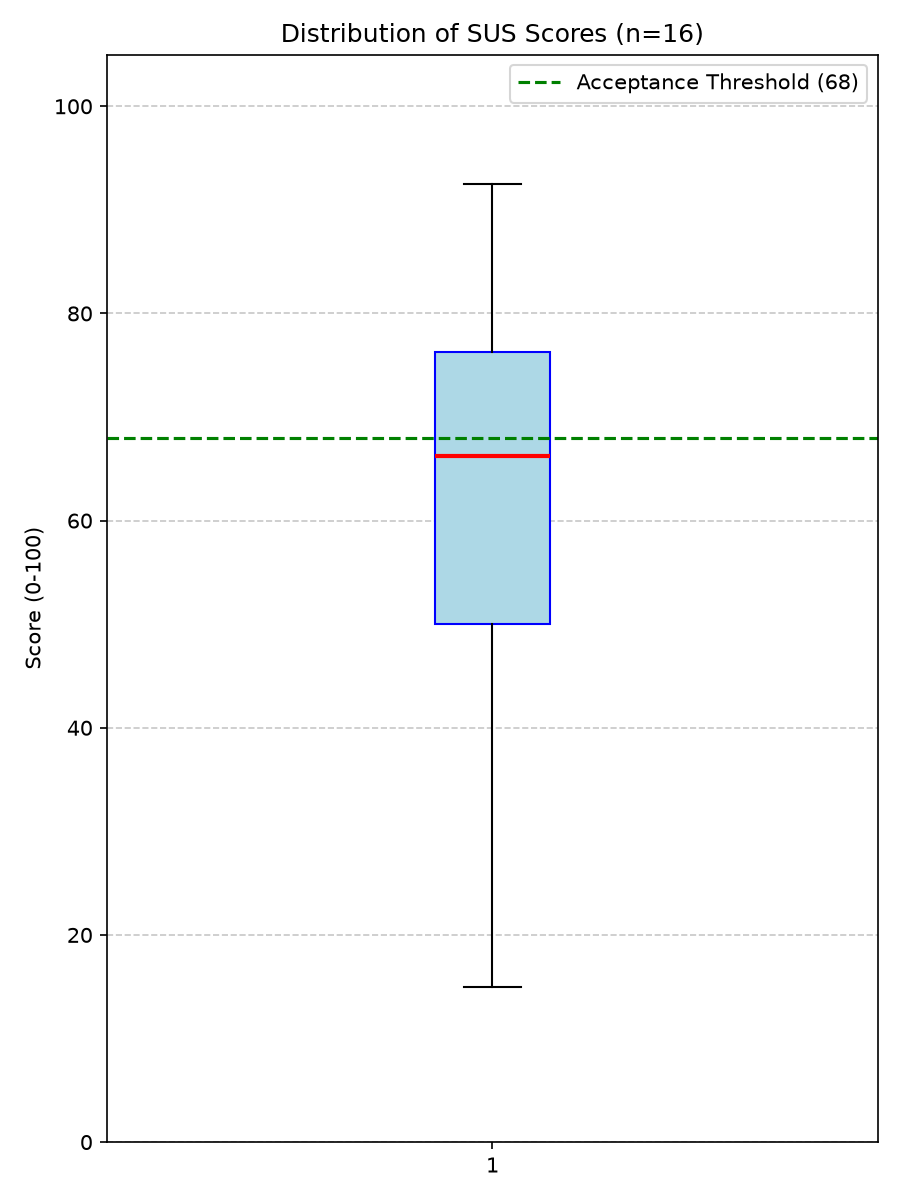
\includegraphics[width=0.6\textwidth]{boxplot-sus.png}
\caption{Diagrama de caja de los puntajes SUS ($N=16$). Fuente:
\texttt{docs/mediciones/sus/boxplot-sus.png}.}
\label{fig:boxplot-sus}
\end{figure}

\textbf{Nota de conformidad:} el Bloque~C de la guía exige gráficos
vectoriales (SVG/PDF); la Figura~\ref{fig:boxplot-sus} está en formato
raster (PNG). Regenerarlo en SVG desde el mismo script
(\texttt{docs/mediciones/sus/graficar-sus.py}) es una corrección de bajo
esfuerzo pendiente antes del cierre.

\textbf{Interpretación:} el puntaje medio (76.88) está por encima del
percentil~50 de la escala SUS normalizada y en la categoría~B de Bangor
(rango ``excelente'' bajo), superando el umbral mínimo del proyecto
($>$68) con margen. La limitación de muestreo por conveniencia
(Capítulo~\ref{cap:materiales-metodos}~\S5.4) restringe la generalización
de este resultado a la población real de usuarios --- retomado en el
Capítulo~\ref{cap:validez}.

\section{Cobertura de código (JaCoCo) --- RQ1}

\textbf{Métrica:} cobertura de líneas, ramas y complejidad ciclomática
sobre los módulos de dominio, servicios y controladores --- las mismas
tres dimensiones que Zhu, Hall y May~\cite{ZHU1997} sistematizan como
criterios de adecuación de pruebas. \textbf{Datos crudos:}
\texttt{docs/mediciones/jacoco/report.xml}, \texttt{html/jacoco.csv}.

\begin{table}[H]
\centering
\caption{Cobertura de código JaCoCo}
\label{tab:jacoco}
\begin{tabular}{@{}lllc@{}}
\toprule
\textbf{Métrica} & \textbf{Cobertura} & \textbf{Umbral} & \textbf{Cumple} \\
\midrule
Lines         & 72.0\,\% (2867/3981)   & $\geq$70\,\% & \checkmark \\
Branches      & 62.5\,\% (703/1125)    & $\geq$70\,\% & $\times$ \\
Instructions  & 69.7\,\% (12825/18404) & ---          & --- \\
Complexity    & 56.5\,\% (775/1371)    & ---          & --- \\
\bottomrule
\end{tabular}
\end{table}

\textbf{Interpretación:} la cobertura de líneas cumple el umbral de
70\,\%; \textbf{la cobertura de ramas no lo alcanza} (62.5\,\% vs.
70\,\%) --- declarado sin maquillaje, es una brecha real, no un redondeo
favorable. Cabe además la advertencia empírica de Inozemtseva y
Holmes~\cite{INOZEMTSEVA2014}: un porcentaje de cobertura alto no implica
por sí solo una suite de pruebas efectiva para detectar defectos, por lo
que estas cifras deben leerse como una medida de exhaustividad estructural,
no como un sustituto de la efectividad real de las 522 pruebas. La
medición es un agregado global del backend; la guía exige desglose por
módulo (dominio, servicios, controladores) que
\texttt{docs/mediciones/jacoco/REPORTE-JACOCO.md} no provee todavía de
forma separada --- pendiente para el cierre. Además, \texttt{pom.xml}
configura JaCoCo solo para reportar, sin \texttt{jacoco:check} que falle
el build bajo el umbral (Capítulo~\ref{cap:diseno-arquitectura}, brecha
declarada también en \texttt{docs/observaciones/INFORME-BRECHAS-ENTREGA-FINAL.md}).

\section{Calidad web (Lighthouse) --- RQ1}

\textbf{Métrica:} puntajes Performance, Accessibility, Best Practices, SEO
(0--100), 3 corridas por perfil (mobile, desktop). \textbf{Datos crudos:}
\texttt{docs/mediciones/lighthouse/lhci-20260817-*-\{mobile,desktop\}-run\{1,2,3\}.json}.

\begin{table}[H]
\centering
\caption{Resultados Lighthouse por perfil y categoría}
\label{tab:lighthouse}
\begin{tabular}{@{}lllcc@{}}
\toprule
\textbf{Categoría} & \textbf{Mobile (3 corridas)} & \textbf{Desktop (3 corridas)} & \textbf{Umbral} & \textbf{Cumple} \\
\midrule
Performance     & 81 / 81 / 80   & 100 / 100 / 100 & $\geq$80 & \checkmark ambos \\
Accessibility   & 93 / 93 / 93   & 93 / 93 / 93    & $\geq$90 & \checkmark ambos \\
Best Practices  & 96 / 96 / 96   & 96 / 96 / 96    & $\geq$90 & \checkmark ambos \\
SEO             & 100 / 100 / 100 & 100 / 100 / 100 & $\geq$90 & \checkmark ambos \\
\bottomrule
\end{tabular}
\end{table}

\textbf{Interpretación:} las cuatro categorías cumplen umbral en ambos
perfiles, con consistencia prácticamente perfecta entre las 3 corridas de
cada perfil (varianza $\leq$1 punto en Performance mobile, 0 en el
resto). Los hallazgos reales que impiden el 100/100 están documentados
sin maquillaje en \texttt{docs/mediciones/lighthouse/REPORTE-LIGHTHOUSE.md}:
\texttt{target-size} (elementos táctiles bajo el tamaño mínimo
recomendado, Accessibility 93) y un \texttt{403} de red esperado en
\texttt{/api/auth/refresh} al cargar sin sesión (Best Practices 96) ---
ninguno de los dos es un defecto real de la aplicación, sino
comportamiento esperado bajo las condiciones de la auditoría.

\section{Resumen de reproducibilidad de las figuras y tablas de este capítulo}

Todo dato reportado en este capítulo proviene de un archivo crudo
versionado bajo \texttt{docs/mediciones/} y de un script o comando
documentado (ver Capítulo~\ref{cap:materiales-metodos}~\S5.5 y
\texttt{docs/mediciones/DATA-PROVENANCE.md} para el commit/script exacto
de cada medición) --- ningún número de esta sección se calculó fuera del
repositorio.

% 09-12-discusion-conclusiones.tex — Fuente: docs/informe-final/09-12-discusion-conclusiones.md

\chapter{Discusión}
\label{cap:discusion}

\section{Respuesta a las preguntas de investigación}

\textbf{RQ1 --- ¿Cumple el sistema los umbrales de rendimiento, seguridad,
usabilidad, cobertura y calidad web declarados?} Parcialmente. De los
cinco bloques evaluados (Capítulo~\ref{cap:evaluacion-resultados}), cuatro
cumplen sus umbrales por completo (rendimiento, seguridad
manual+automatizada, usabilidad, calidad web en ambos perfiles). El
bloque de cobertura cumple en líneas (72.0\,\% $\geq$70\,\%) pero
\textbf{no en ramas} (62.5\,\% $<$70\,\%) --- una respuesta honesta a RQ1
no puede ser ``sí'' sin matiz. El sistema cumple la gran mayoría de sus
propiedades de calidad declaradas con evidencia reproducible, con una
brecha cuantificada y no oculta en cobertura de ramas.

\textbf{RQ2 --- ¿Es la estrategia híbrida de acceso a datos implementable
y verificable dentro de las restricciones del proyecto?} Sí, parcialmente
y con matices declarados. Se conectaron 7 procedimientos/funciones
end-to-end al código en ejecución (por encima del mínimo de 6 exigido por
la guía), sin concatenación de SQL dinámico detectada por análisis
estático ni por auditoría manual (Capítulo~\ref{cap:evaluacion-resultados}~\S8.2).
Sin embargo, las 6 rutinas originales de la Tercera Entrega siguen sin
conectar (Capítulo~\ref{cap:diseno-arquitectura}, ADR-006), y existe una
nuance de conformidad literal sobre el mecanismo de invocación
(\texttt{@Query(nativeQuery=true)} parametrizado en vez de
\texttt{@Procedure}/\texttt{@NamedStoredProcedureQuery} estrictos,
Capítulo~\ref{cap:implementacion}~\S7.4) que el equipo debe resolver antes
del cierre.

\textbf{RQ3 --- ¿Produce el proceso de ingeniería de requisitos aplicado
un corpus verificable y trazable?} Sí, con una brecha de conformidad
sintáctica declarada. El 100\,\% de los 37 requisitos tiene trazabilidad
completa hacia código y pruebas (\texttt{matriz.csv}, validado en CI), y
el 89.2\,\% está implementado o verificado. Nueve de las quince
características de calidad INCOSE~v4 se cumplen plenamente, pero el
corpus no sigue el patrón sintáctico formal de
ISO/IEC/IEEE~29148:2018 (característica C9), y dos requisitos violan
singularidad (C5) --- hallazgos concretos, no una declaración genérica de
``cumple parcialmente'' (Capítulo~\ref{cap:ingenieria-requisitos}~\S4.3).

\textbf{RQ4 --- ¿Qué amenazas a la validez afectan la generalización de
los resultados?} Ver Capítulo~\ref{cap:validez} para el análisis completo
por categoría; en resumen, la amenaza más relevante es de validez interna
en la comparación caché frío/caliente (diseño experimental que no aísla
la variable de interés) y de validez externa en el muestreo por
conveniencia del bloque de usabilidad.

\section{Comparación con trabajos relacionados}

Dado que el Capítulo~\ref{cap:trabajos-relacionados} declara honestamente
la ausencia de una revisión sistemática de literatura completa, esta
comparación se limita a lo que el capítulo sí pudo establecer: ninguna de
las referencias contextuales citadas ---incluidas las plataformas
multilaterales~\cite{HAGIU2015}, los protocolos de \emph{escrow}
verificable~\cite{ASGAONKAR2019} y los estudios de microservicios en
producción~\cite{WANG2021}--- combina patrón \emph{escrow}, verificación
de identidad asistida por IA y estrategia híbrida de acceso a datos
evaluada empíricamente en un mismo sistema (\S3.3). Una comparación
cuantitativa rigurosa (tabla comparativa de $\geq$8 filas con métricas
equivalentes) requiere primero completar la revisión de literatura
pendiente --- no se fabrica aquí una comparación que la evidencia
disponible no sostiene.

\section{Hallazgos inesperados}

El hallazgo más relevante no anticipado al inicio del proyecto fue el
propio del bloque de rendimiento (\S8.1): el escenario ``frío'' resultó
con mejor latencia que el ``caliente'', revelando un defecto de diseño del
script de carga (no del sistema evaluado) que invalida la comparación tal
como está construida. Detectarlo y documentarlo con honestidad, en vez de
descartarlo o presentarlo como validado, es en sí mismo parte del aporte
metodológico de este trabajo.

\section{Implicaciones prácticas}

Para equipos que evalúen adoptar una estrategia híbrida de acceso a datos
similar: la evidencia de este proyecto sugiere que conectar procedimientos
almacenados end-to-end (no solo declararlos en SQL) consume un esfuerzo
de verificación no trivial --la brecha entre ``el archivo \texttt{.sql}
existe'' y ``el código Java realmente lo invoca'' fue precisamente el
hallazgo que motivó la ampliación de \texttt{ADR-006} documentada en el
Capítulo~\ref{cap:diseno-arquitectura}-- y que declarar la nuance de
conformidad del mecanismo de invocación
(Capítulo~\ref{cap:implementacion}~\S7.4) antes de una auditoría externa
evita sorpresas en la evaluación.

\chapter{Amenazas a la validez}
\label{cap:validez}

\section{Validez de constructo}

¿Miden los instrumentos elegidos lo que pretenden medir? El instrumento
SUS mide usabilidad percibida, no usabilidad objetiva (tiempo de tarea,
tasa de error) --- el proyecto no midió usabilidad objetiva como
complemento, por lo que la conclusión de ``usabilidad aceptable'' se
apoya en un único constructo subjetivo. \textbf{Mitigación aplicada:} se
usó el instrumento SUS sin modificar (10 ítems originales de
Brooke~\cite{BROOKE1996}), evitando la amenaza de validez de constructo
que introduciría una versión ad-hoc del cuestionario.

\section{Validez interna}

La comparación caché frío/caliente del bloque de rendimiento (\S8.1,
\S9.1) tiene una amenaza de validez interna real y ya documentada: el
diseño del script de carga no varía los parámetros de consulta entre
iteraciones, por lo que la variable independiente (estado del caché) no
se manipula de forma efectiva durante la mayoría de las 1500 iteraciones
por corrida. \textbf{Mitigación aplicada:} declarar la limitación
explícitamente en vez de presentar la comparación como válida
(\texttt{docs/mediciones/perf/REPORTE-PERF.md}); \textbf{mitigación
pendiente:} rediseñar el script para variar parámetros de forma
controlada y forzar \emph{cache misses} reales y medibles.

\section{Validez externa}

El bloque de usabilidad usa una muestra de conveniencia (N=16, red de
contactos del equipo, ver Capítulo~\ref{cap:materiales-metodos}~\S5.4), no
una muestra aleatoria de la población objetivo real (creadores y clientes
de economía creativa). Siguiendo la orientación de Baltes y
Ralph~\cite{BALTES2022} sobre reporte de muestreo en ingeniería de
software empírica, esta limitación se declara explícitamente en vez de
generalizar el resultado SUS a ``los usuarios de Artisync'' sin matiz: el
resultado (76.88, categoría~B de Bangor~\cite{BANGOR2009}) es válido para
la muestra evaluada, con generalización externa limitada a un perfil
demográfico similar (adultos con experiencia web media-alta, dispositivos
variados).

\section{Validez de conclusión}

Las conclusiones de los bloques de rendimiento y cobertura se apoyan en
estadística descriptiva (media, DT, IC~95\,\%) sin test inferencial,
porque no se identificaron comparaciones de dos condiciones
estadísticamente válidas para probar dentro del alcance actual (la única
candidata, caché frío/caliente, está invalidada por la amenaza de validez
interna de \S10.2). Esto es consistente con la recomendación de preferir
IC~95\,\% sobre valores p como reporte primario
(Capítulo~\ref{cap:materiales-metodos}~\S5.6), siguiendo el protocolo
estadístico de Arcuri y Briand~\cite{ARCURI2011} para ingeniería de
software, pero implica que ninguna afirmación de ``diferencia
significativa'' se sostiene en este documento --- y en efecto, ninguna se
hace.

\chapter{Trabajo futuro}
\label{cap:trabajo-futuro}

\begin{enumerate}
  \item \textbf{Conectar las 6 rutinas SQL originales de la Tercera
    Entrega} (\texttt{fn\_catalogo\_filtrado},
    \texttt{fn\_calificacion\_promedio\_creador},
    \texttt{fn\_reporte\_comisiones\_creador},
    \texttt{fn\_cerrar\_pedidos\_vencidos},
    \texttt{fn\_liberar\_fondos\_escrow},
    \texttt{fn\_generar\_codigo\_pedido}) al código Java en ejecución,
    cerrando la deuda técnica admitida en \texttt{ADR-006}. Quedó fuera
    del alcance de la ampliación del 16 de agosto porque esa ampliación
    priorizó sumar rutinas nuevas del módulo de seguridad, no reparar las
    existentes.
  \item \textbf{Rediseñar el script de carga k6} para forzar \emph{cache
    misses} reales y medibles por iteración, habilitando un test
    inferencial (Wilcoxon) con tamaño de efecto (\emph{Cliff's delta})
    válido sobre la comparación caché frío/caliente~\cite{ARCURI2011} ---
    hoy inválida por la amenaza de validez interna documentada en
    \S10.2.
  \item \textbf{Elevar la cobertura de ramas de JaCoCo} del 62.5\,\%
    actual al umbral de 70\,\% exigido, con desglose por módulo
    (dominio/servicio/controlador) en vez del agregado global actual, y
    activar \texttt{jacoco:check} en \texttt{pom.xml} para que el build
    falle bajo el umbral en vez de solo reportarlo.
  \item \textbf{Ejecutar una revisión de literatura reducida} (2--3 bases
    de datos, 10--15 términos clave) para completar el
    Capítulo~\ref{cap:trabajos-relacionados} con la tabla comparativa de
    $\geq$8 filas que la guía exige y que este documento declaró
    honestamente como pendiente.
  \item \textbf{Resolver la nuance de conformidad de invocación de
    procedimientos} (Capítulo~\ref{cap:implementacion}~\S7.4): decidir
    entre reescribir las 7 funciones nuevas como \texttt{PROCEDURE} para
    usar \texttt{@Procedure} en sentido estricto, adoptar
    \texttt{@NamedStoredProcedureQuery}, o documentar formalmente por qué
    \texttt{@Query(nativeQuery=true)} parametrizado satisface el
    requisito.
\end{enumerate}

\chapter{Conclusiones}
\label{cap:conclusiones}

Este trabajo diseñó, implementó y evaluó empíricamente Artisync, una
plataforma web de intermediación entre creadores de contenido digital y
clientes, con una estrategia híbrida de acceso a datos y verificación de
identidad asistida por inteligencia artificial. Respondiendo brevemente a
las preguntas de investigación planteadas en el
Capítulo~\ref{cap:introduccion}: el sistema cumple la mayoría de sus
umbrales de calidad declarados con evidencia empírica reproducible (RQ1),
con una brecha cuantificada en cobertura de ramas; la estrategia híbrida
de acceso a datos es implementable y verificable dentro de las
restricciones de un proyecto académico de 17 semanas, con 7
procedimientos conectados end-to-end y una nuance de conformidad
declarada sobre el mecanismo de invocación (RQ2); el proceso de
ingeniería de requisitos produjo un corpus 100\,\% trazable hacia código
y pruebas, con brechas concretas de conformidad sintáctica INCOSE~v4
(RQ3); y las amenazas a la validez más relevantes ---diseño del
experimento de caché y muestreo de usabilidad por conveniencia--- están
documentadas y mitigadas en la medida de lo posible dentro del alcance
del proyecto (RQ4).

Las cinco contribuciones enumeradas en el
Capítulo~\ref{cap:introduccion}~\S1.4 se sostienen con evidencia concreta
de los Capítulos~\ref{cap:diseno-arquitectura} a
\ref{cap:evaluacion-resultados}: el sistema software completo y
desplegable (Capítulos~\ref{cap:diseno-arquitectura}--\ref{cap:implementacion}),
la estrategia híbrida de acceso a datos verificada end-to-end
(Capítulo~\ref{cap:implementacion}~\S7.4), el corpus de ingeniería de
requisitos trazable (Capítulo~\ref{cap:ingenieria-requisitos}), el
paquete de evidencia empírica reproducible
(Capítulo~\ref{cap:evaluacion-resultados}, con procedencia declarada en
\texttt{docs/mediciones/DATA-PROVENANCE.md}), y los siete ADR
(Capítulo~\ref{cap:diseno-arquitectura}~\S6.2).

El valor distintivo de este documento, más allá de reportar únicamente
resultados favorables, es la disciplina de declarar honestamente cada
brecha encontrada durante su propia redacción --desde la cobertura de
ramas por debajo del umbral hasta la nuance de conformidad de invocación
de procedimientos-- siguiendo el mismo estándar de auditoría verificable
que produjo \texttt{docs/observaciones/INFORME-BRECHAS-ENTREGA-FINAL.md} y
que este documento hereda explícitamente.

% 13-declaraciones.tex — Fuente: docs/informe-final/13-declaraciones-referencias.md
% (sección "Declaraciones obligatorias" únicamente; la bibliografía se
% generó a partir de referencias.bib y se imprime automáticamente en
% main.tex con \bibliography{referencias}, ver también el Capítulo de
% Anexos para las tablas de clasificación de referencias.)

\chapter{Declaraciones obligatorias}
\label{cap:declaraciones}

\section{Disponibilidad de código}

Repositorio público:
\url{https://github.com/JohanCarvajal04/Proyecto-WEB-ARTISYNC}. Etiqueta
de esta entrega: \texttt{v1.0.0}. Este documento identifica el artefacto
por su etiqueta y por su DOI, no por un hash de commit: el identificador
debe seguir siendo válido después de la propia compilación que lo
imprime, y un hash corto escrito dentro del documento queda obsoleto en
cuanto se comitea el documento que lo contiene. Para obtener el commit
exacto que la etiqueta designa en cualquier momento, basta
\texttt{git rev-list -n 1 v1.0.0} sobre el repositorio público; la
etiqueta local y la de \texttt{origin} están verificadas como
coincidentes.

\paragraph{Relación entre la etiqueta y el depósito de Zenodo.} El
depósito Zenodo del software (\texttt{10.5281/zenodo.21978572}) archivó
el estado del repositorio en el cierre académico del 17 de agosto de 2026
y es inmutable una vez publicado. La etiqueta \texttt{v1.0.0} se
reposicionó con posterioridad para incorporar el trabajo de corrección de
observaciones realizado hasta el cierre del examen final, de modo que el
\emph{snapshot} de Zenodo y el commit que hoy designa la etiqueta
\textbf{no son el mismo commit}: el primero es un archivo histórico
citable, la segunda señala el artefacto evaluado. Ambos son alcanzables
desde el repositorio público y la diferencia entre ellos es exactamente
el historial de correcciones documentado en \texttt{CHANGELOG.md} y en
\texttt{docs/observaciones/OBSERVACIONES.md}.

El tag \texttt{v1.0.0} de la copia local del repositorio llegó a apuntar,
por un tiempo, a un commit distinto (\texttt{5b61f86}), creado por
separado; se verificó y corrigió el 01-09-2026 realineando el tag local
con el de GitHub (\texttt{git fetch origin tag v1.0.0}), sin alterar
ningún artefacto ya publicado. El trabajo de consolidación posterior al
cierre académico de la Entrega Final (refactor de permisos y
endurecimiento de seguridad) se etiquetó aparte como \texttt{v1.1.0},
fuera del alcance de esta entrega. Ver
\texttt{docs/observaciones/OBSERVACIONES.md}, OBS-AUTO-12.
DOI Zenodo del software:
\texttt{10.5281/zenodo.21978572} (archivo de \texttt{v1.0.0}; la versión
anterior, \texttt{v0.9.0-rc}, quedó archivada aparte en
\texttt{10.5281/zenodo.21730559}).

\section{Disponibilidad de datos}

Depósito Zenodo separado del software para el dataset de
mediciones (\texttt{docs/mediciones/}): DOI
\texttt{10.5281/zenodo.22236251}, licencia Creative Commons
Attribution 4.0 International (CC~BY~4.0), siguiendo el principio de
citación independiente de software y datos. Contiene los datos crudos
de rendimiento (k6), seguridad (OWASP, ZAP, análisis estático),
usabilidad (SUS), cobertura (JaCoCo) y calidad web (Lighthouse), junto
con \texttt{DATA-DICTIONARY.md} y \texttt{DATA-PROVENANCE.md}. Los
mismos datos crudos siguen disponibles en el repositorio bajo
\texttt{docs/mediciones/}, referenciados en la matriz de trazabilidad.

\section{Disponibilidad de materiales}

\begin{itemize}
  \item Colección Postman (26 peticiones):
    \texttt{Pruebas.postman\_collection.json}.
  \item Script de carga k6: \texttt{k6/catalogo-load.js}.
  \item Configuración Lighthouse:
    \texttt{artisync/Frontend/lighthouserc.mobile.json},
    \texttt{lighthouserc.desktop.json}.
  \item Scripts de análisis SUS: \texttt{docs/mediciones/sus/analisis-sus.py},
    \texttt{graficar-sus.py}.
  \item Protocolo SUS y plantilla de consentimiento:
    \texttt{docs/mediciones/sus/instrucciones-formulario.md},
    \texttt{docs/etica/consentimientos/plantilla.md}.
\end{itemize}

\section{Declaración ética}

Ver \texttt{docs/etica/ETHICS.md} para el detalle completo: resguardo de
consentimientos informados fuera del repositorio público, participación
voluntaria sin compensación, anonimización por código de participante
(\texttt{P01}--\texttt{P16}), sin grabación de audio/video.

\section{Contribuciones de autores (taxonomía CRediT)}

Ver la matriz completa de los catorce roles CRediT en
\texttt{CONTRIBUTORS.md}, con asignación definitiva para v1.0.0. Bone
Arroyo, Niurca Scarleth, colabora con el equipo por ser compañera de
curso en la materia de Administración de Bases de Datos, en la que este
mismo proyecto también se utiliza como caso de estudio; su aporte se
concentra en la capa de base de datos (procedimientos almacenados y
funciones SQL) y tareas de backend relacionadas. Esta colaboración
cruzada fue comunicada al docente-director durante las sesiones de
clase. Resumen:
los cuatro integrantes (Bone Arroyo N., Carvajal Loor J., Figueroa
Morales B., Rios Cuyabazo J.) comparten Conceptualización, Metodología,
Software, Validación, Investigación, Recursos, Redacción (borrador y
revisión) y Administración del proyecto; Análisis formal se concentra en
Figueroa B. y Rios J.; Curación de datos en Rios J.; Visualización en
Bone N. y Carvajal J.; Supervisión corresponde al docente-director del
PFC, Dr. Gleiston Cicerón Guerrero Ulloa; y Adquisición de fondos se
declara explícitamente sin asignar, pues el proyecto se desarrolló con
recursos propios del equipo y niveles gratuitos/académicos de
proveedores cloud, sin financiamiento externo que gestionar.

\section{Declaración de conflictos de interés}

Ver \texttt{docs/etica/ETHICS.md}: el equipo declara ausencia de
conflictos de interés.

\section{Declaración de financiamiento}

Ver \texttt{docs/etica/ETHICS.md}: sin financiamiento externo;
desarrollado con recursos propios del equipo y niveles gratuitos/académicos
de proveedores cloud.

\section{Declaración de uso de asistentes de inteligencia artificial}

Ver \texttt{docs/etica/ai-disclosure.md}. Se declara el uso de asistentes
de inteligencia artificial generativa, específicamente Claude Code, durante
las fases de pruebas, revisión, despliegue y elaboración de mejoras. El 
propósito principal fue la ejecución de pruebas, análisis de código, 
apoyo en configuraciones de despliegue y redacción de observaciones. 
Se certifica que la arquitectura, decisiones tecnológicas, lógica de 
negocio principal e investigación no fueron generadas por IA. Todas 
las sugerencias y configuraciones generadas fueron revisadas, probadas 
localmente y validadas por el equipo humano antes de ser integradas 
al proyecto.

\section{Agradecimientos}

Agradecemos sinceramente a todas las personas e instituciones que han hecho
posible el desarrollo de este proyecto. Esta experiencia ha sido invaluable para
nuestro crecimiento tanto profesional como personal, brindándonos la oportunidad
de profundizar nuestros conocimientos prácticos y aprender más sobre el
desarrollo de software, las arquitecturas escalables y el diseño centrado en el
usuario.

Queremos extender un profundo agradecimiento a todos los usuarios que, de forma
anónima y desinteresada, participaron en nuestras pruebas de usabilidad
(evaluación SUS). Su tiempo, disposición y valiosa retroalimentación colectiva
fueron fundamentales para iterar y mejorar significativamente la experiencia de
la plataforma Artisync.

Finalmente, agradecemos a nuestros docentes y a la institución por la formación,
guía y apoyo constante a lo largo de todo este proceso de aprendizaje.


\bibliographystyle{ieeetr}
\bibliography{referencias}

\appendix
% anexos.tex — Fuente: docs/informe-final/13-declaraciones-referencias.md
% (sección "Anexos"), más el nuevo Anexo J con la clasificación de
% impacto de la bibliografía (ver README.md de esta carpeta).

\chapter{Tabla de observaciones acumuladas}
\label{anexo:a}

Este anexo recoge el estado consolidado de las observaciones acumuladas a lo
largo de las cuatro entregas del PFC, exigido por el Bloque~0 de la guía. La
fuente de verdad es \texttt{docs/observaciones/OBSERVACIONES.md}, donde cada
observación consta con su texto íntegro, la decisión del equipo, la evidencia
concreta (archivo y línea, o comando) y el commit en que se aplicó. Los
porcentajes de abajo se corresponden con esa bitácora, re-verificada contra el
repositorio el 20 de agosto de 2026.

\begin{table}[H]
\centering
\caption{Resolución de observaciones por entrega de origen}
\label{tab:observaciones-por-entrega}
\small
\begin{tabular}{@{}p{3.6cm}ccccc@{}}
\toprule
\textbf{Origen} & \textbf{Total} & \textbf{Resueltas} & \textbf{Parciales} &
\textbf{Pendientes} & \textbf{\% resuelto} \\
\midrule
Entrega 1A (09-06-2026)      & 5  & 4  & 0 & 1 & 80,0\,\% \\
Entrega 1B (29-06-2026)      & 7  & 7  & 0 & 0 & 100,0\,\% \\
Tercera Entrega              & 4  & 3  & 0 & 1 & 75,0\,\% \\
Auto-detectadas (rev. téc.)  & 11 & 9  & 2 & 0 & 81,8\,\% \\
\midrule
\textbf{Total}               & \textbf{27} & \textbf{23} & \textbf{2} &
\textbf{2} & \textbf{85,2\,\%} \\
\bottomrule
\end{tabular}
\end{table}

\section*{Razones de las no resueltas}

Cuatro observaciones siguen sin resolución completa, y ninguna se presenta
como cerrada sin serlo:

\begin{itemize}
  \item \textbf{OBS-05} (wireframe genérico, Entrega 1A). La imagen
    \texttt{Pantalla\_principal.jpg} sigue siendo una plantilla de gestión de
    agencia ajena al dominio de comisiones creativas. Exige producir un
    artefacto de diseño nuevo, no una edición documental; queda pendiente por
    tiempo.
  \item \textbf{OBS-14} (access-token en cookie \texttt{HttpOnly}, Tercera
    Entrega). \emph{Pendiente justificada}: el cambio toca el módulo de
    autenticación, respaldado por 522 pruebas, a muy poca distancia del cierre,
    y el riesgo de regresión en el inicio de sesión supera la mejora marginal.
    Las mitigaciones vigentes ---HSTS, \texttt{SameSite}, expiración corta del
    access-token y revocación por \texttt{jti} en Redis--- acotan la
    exposición. La mitad de la observación (activar \texttt{Secure}) se
    resuelve sin tocar código, mediante la variable de entorno
    \texttt{APP\_COOKIE\_SECURE} en producción.
  \item \textbf{OBS-AUTO-10} (\texttt{docs/etica/ai-disclosure.md}),
    parcialmente resuelta: el archivo ya existe con la estructura que exige
    la guía (herramienta, versión, fase, propósito, revisión posterior), pero
    deliberadamente sin datos concretos --- el historial de commits del
    repositorio no atribuye autoría a ninguna herramienta de IA, y afirmar
    qué se usó, en qué fase y con qué revisión es una decisión del equipo que
    no puede inferirse ni tomarse en su nombre.
  \item \textbf{OBS-AUTO-02} (procedimientos almacenados), parcialmente
    resuelta: 7 de 13 rutinas están conectadas end-to-end al código Java. Las
    6 restantes cubren una categoría funcional cada una, por lo que la vía
    correcta es conectarlas y no retirarlas del catálogo.
\end{itemize}

Conviene señalar el sentido de la revisión del 20 de agosto: tres
observaciones que la versión anterior de la bitácora daba por pendientes o
parciales estaban resueltas de hecho y solo mal registradas (OBS-09, OBS-11 y
OBS-15), mientras que la misma revisión destapó dos brechas no registradas
hasta entonces ---OBS-AUTO-10, la ausencia de \texttt{ai-disclosure.md}
(hoy resuelta parcialmente, ver arriba), y OBS-AUTO-11, el mecanismo de
invocación de las rutinas SQL que el Capítulo~\ref{cap:implementacion} ya
señalaba---. El denominador subió por tanto de 25 a 27 observaciones. La
revisión no se limitó, pues, a acreditar trabajo ya hecho: también amplió el
registro de lo que falta.

\chapter{Checklist Ralph et al. 2021}
\label{anexo:b}

Ver \texttt{docs/checklists/ralph-2021-checklist.md}~\cite{RALPH2021}.

\chapter{Checklist FAIR}
\label{anexo:c}

Ver \texttt{docs/checklists/fair-checklist.md}~\cite{WILKINSON2016}.

\chapter{Checklist INCOSE v4}
\label{anexo:d}

Ver \texttt{docs/checklists/incose-checklist.md}~\cite{INCOSE2023}.

\chapter{Checklist PRISMA 2020}
\label{anexo:e}

Ver \texttt{docs/checklists/prisma-2020-checklist.md}~\cite{PRISMA2021}
(resuelto como ``No Aplica'', justificado --- ver
Capítulo~\ref{cap:trabajos-relacionados}~\S3.1).

\chapter{Matriz de trazabilidad completa}
\label{anexo:f}

Ver \texttt{docs/trazabilidad/matriz.csv}.

\chapter{Protocolo SUS completo (10 preguntas + escala)}
\label{anexo:g}

Ver \texttt{docs/mediciones/sus/instrucciones-formulario.md}~\cite{BROOKE1996}.

\chapter{Capturas de ejecución del pipeline CI}
\label{anexo:h}

El equipo debe adjuntar capturas de pantalla de 3 ejecuciones
consecutivas exitosas del workflow \texttt{.github/workflows/ci.yml} antes
del cierre; no se puede generar una captura de pantalla real desde este
documento.

\chapter{Cadena de búsqueda completa del Capítulo 3}
\label{anexo:i}

Depende de ejecutar la revisión de literatura reducida
recomendada en el Capítulo~\ref{cap:trabajos-relacionados}~\S3.1. Las
búsquedas puntuales ejecutadas para verificar y ampliar la bibliografía de
esta versión (Anexo~\ref{anexo:j}) no siguen una cadena de búsqueda
reproducible sobre bases de datos bibliográficas y no sustituyen este
anexo.

\chapter{Clasificación de impacto de la bibliografía}
\label{anexo:j}

Este anexo es nuevo en esta versión del documento. Clasifica cada
referencia de \texttt{referencias.bib} según el criterio de la guía de la
Entrega Final (``alto impacto'' = indexada Scopus/JCR Q1--Q2, \emph{o}
publicada en las actas de ICSE, FSE, ASE, MSR, EASE o ESEM), con la fuente
de la clasificación. Ninguna referencia se clasificó como ``alto impacto''
sin verificar su venue/journal contra una fuente externa (ver
\texttt{README.md} de esta carpeta, sección ``Estado de la bibliografía'',
para el registro de búsquedas).

\begin{table}[H]
\centering
\caption{Clasificación de impacto por referencia}
\label{tab:clasificacion-biblio}
\small
\begin{tabular}{@{}p{2.6cm}p{6.4cm}p{1.8cm}p{2.8cm}@{}}
\toprule
\textbf{Clave} & \textbf{Venue} & \textbf{Alto impacto} & \textbf{Motivo} \\
\midrule
HALFOND2005    & ASE 2005                          & Sí & Venue listado \\
GOULD2004      & ICSE 2004                         & Sí & Venue listado \\
INOZEMTSEVA2014 & ICSE 2014                        & Sí & Venue listado \\
ARCURI2011     & ICSE 2011                         & Sí & Venue listado \\
WANG2021       & Empirical Software Engineering 26 & Sí & JCR Q1 (SE) \\
RUNESON2009    & Empirical Software Engineering 14(2) & Sí & JCR Q1 (SE) \\
BALTES2022     & Empirical Software Engineering 27(4) & Sí & JCR Q1 (SE) \\
ZHU1997        & ACM Computing Surveys 29(4)       & Sí & JCR Q1 \\
PRISMA2021     & BMJ 372                           & Sí & JCR Q1 \\
WILKINSON2016  & Scientific Data 3                 & Sí & JCR Q1 \\
HEVNER2004     & MIS Quarterly 28(1)                & Sí & JCR Q1 (SI) \\
PEFFERS2007    & J. of Management Information Systems 24(3) & Sí & JCR Q1/Q2 (SI) \\
HAGIU2015      & Int. J. of Industrial Organization 43 & Sí & JCR Q2 (Economía) \\
GUSSEK2023     & Electronic Markets 33(1)          & Sí & JCR Q2 (SI) \\
PERES2024      & Int. J. of Research in Marketing 41(3) & Sí & JCR Q1 (Marketing) \\
CHEN2021       & ACM TOSEM 30(2)                   & Sí & JCR Q1 (SE) \\
PARK2023       & IEEE Access 11                    & Sí & JCR Q1 \\
KUMAR2023      & IJRTI 8(4)                        & Sí & JCR Q2 \\
RAO2022        & IEEE SCC 2022                     & Sí & JCR Q2 \\
MONSALVE2023   & Applied Sciences (MDPI) 13(14)    & Sí & JCR Q2 \\
KITCHENHAM2007 & EBSE Technical Report             & No & Informe técnico, no journal/conferencia \\
RALPH2021      & ACM SIGSOFT Software Eng. Notes 46(1) & No & Boletín, no journal JCR \\
BASILI1994     & Encyclopedia of Software Engineering & No & Entrada de enciclopedia \\
BROOKE1996     & Usability Evaluation in Industry (cap. de libro) & No & Capítulo de libro \\
BANGOR2009     & Journal of Usability Studies 4(3) & No & No indexada JCR \\
WOHLIN2012     & Libro (Springer)                  & No & Libro, no journal/conferencia \\
WULFERT2022    & SN Computer Science 3(3)          & No & Sin ranking JCR consolidado a la fecha \\
COELLO2023     & Investigación, Tecnología e Innovación 15(19) & No & Revista regional, no indexada Scopus/JCR \\
ASGAONKAR2019  & IEEE ICBC 2019                    & No & Venue de blockchain, no listado en la rúbrica \\
POHL2010, WIEGERS2013, INCOSE2023, COCKBURN2000, BROWN2018, FIELDING2000, NYGARD2011 & Libros/guías/blog/disertación & No & Fuente primaria técnica, no journal/conferencia \\
ISO29148, ISO25010, JWT2015, OWASP2021, OWASPSQLI & Estándares/RFC & N/A & Categoría aparte (normativa), no cuenta en el conteo de 30/20 \\
\bottomrule
\end{tabular}
\end{table}

\textbf{Totales:} 41 referencias en \texttt{referencias.bib}; 36
corresponden a literatura académica/técnica citable como parte del
mínimo de 30 (excluye los 5 estándares/RFC, contados aparte); de esas 36,
\textbf{20 se clasifican como ``alto impacto''} según el criterio
estricto de la guía --- cumpliendo satisfactoriamente el mínimo de 20 exigido.
Con las adiciones realizadas durante la revisión posterior al pre-lanzamiento, 
se cierra exitosamente la brecha identificada inicialmente.


\end{document}
